\minitoc
\begin{refsection}
\newpage
\fbox{\begin{minipage}{\textwidth}
    \textbf{Contexte :}\\
    Nous avons vu au chapitre \ref{chap:1-particules} que l'observation du processus BWL en laboratoire nécessite la production de photons dans la gamme du MeV ou plus. Ceux-ci pourraient en principe être générés par les processus Compton inverse linéaire, Compton inverse multi-photon ou Bremsstrahlung. Dans ce cadre, les lasers pourraient alors être des outils privilégiés pour la production de telles sources.
    
    \medskip
    \textbf{Résumé du chapitre :}\\
    Dans ce chapitre, les grands principes de production du rayonnement laser sont présentés. Il est ensuite montré que les lasers dits de haute puissance sont principalement produits par deux technologies de milieu amplificateurs, donnant lieu à des énergies, des durées d'impulsion et des taux de répétition différents (figure \ref{fig:2-techno_laser}). Dans le cadre de cette thèse, nous nous concentrerons particulièrement sur les lasers de milieu amplificateur titane-saphire, d'énergie dans la gamme du Joule, de quelques dizaines de femto-secondes de durée et de taux de répétition autour du Hertz. Quelques uns des principaux phénomènes de l'interaction laser-plasma relativiste sont ensuite présentés, dont notamment les phénomènes d'écrantage, d'oscillation plasma, d'ionisation par effet de champ, de transparence induite, d'auto-focalisation relativiste et de force pondéromotrice. Ces informations peuvent alors permettre de comprendre qualitativement quelques uns des mécanismes d'accélération d'électrons par une impulsion laser. Le principe de l'accélération par sillage dans le régime de la bulle (figure \ref{fig:2-acceleration_sillage}), de l'accélération laser directe (figure \ref{fig:2-acceleration_sillage}) ainsi que de l'accélération $\vec{v}\times\vec{B}$ (figure \ref{fig:2-acceleration_magnetique}) sont ensuite discutés. Finalement, quatre schémas de principe permettant de produire des photons de quelques MeV par laser sont présentés (figure \ref{fig:2-config_gamma_laser}), et les caractéristiques principales des sources de photons produites sont illustrées avec des modèles simples, ainsi qu'avec des données expérimentales ou numériques de la littérature. 

    \medskip
    \textbf{Informations complémentaires :}\\
    Une introduction générale sur les lasers peut être trouvée dans la référence \parencite{hennequin_2013}, et le régime haute puissance est plus spécifiquement présenté dans \parencite{danson_2019}. Une introduction générale à la physique des plasmas est quant à elle disponible dans l'ouvrage \parencite{rax_2007}, et le domaine plus spécifique de l'interaction laser-plasma dans le régime relativiste est abordé dans \parencite{macchi_2012, gibbon_2013}. Une discussion sur les effets de l'électrodynamique quantique dans l'interaction laser-matière est disponible dans les articles \parencite{dipiazza_2012, zhang_2020}. Plus d'informations sur l'accélération d'électrons par laser peuvent être trouvées dans la référence \parencite{macchi_2012}, ainsi que dans \parencite{esarey_2009} pour la partie accélération par sillage. Le mécanisme d'accélération directe est détaillé dans l'article \parencite{arefiev_2016}, et le processus $\vec{v}\times\vec{B}$ dans la référence \parencite{wilks_1992}. Une revue de la production de photons dans la gamme keV-MeV en considérant des sources d'électrons accélérés par sillage laser est disponible dans la référence \parencite{albert_2016}, et une revue des sources de rayonnement dans le domaine du keV produites par laser dans la référence \parencite{corde_2013a}.
\end{minipage}}
\newpage

\section{Notions d'interaction laser-plasma relativiste}

Dans cette section, nous présenterons tout d'abord quelques notions de physique du laser nécessaires à la compréhension de la suite de ce manuscrit. Nous discuterons ensuite de quelques comportements généraux des plasmas, puis nous concentrerons principalement sur les plasmas produits par laser, dans le régime relativiste. Cet exposé nous servira de base pour pouvoir comprendre les mécanismes d'accélération d'électrons exposés en section suivante.

\subsection{Notions de physique du laser}

\subsubsection{Remarques générales}

Depuis la production du premier laser à rubis par Maïman en 1960 \parencite{hennequin_2013}, ces derniers ont connu de nombreux développements qui leur ont permis d'atteindre une grande diversité, autant en terme d'énergie que de longueur d'onde, de durée d'impulsion ou de taux de répétition. Un aperçu de cette diversité est illustré en figure \ref{fig:2-diversite_laser}.

\begin{figure}[htbp]
    \centering
    \includegraphics[width=\linewidth]{2-laser/Commercial_laser_lines.png}
    \caption{Illustration des différents types de lasers, en fonction de leur longueur d'onde, énergie de l'impulsion ou puissance continue. Source : Wikipédia, utilisateur Danh, CC-BY-SA (\href{https://en.wikipedia.org/wiki/List_of_laser_types}{https://en.wikipedia.org/wiki/List\_of\_laser\_types}).}
    \label{fig:2-diversite_laser}
\end{figure}

Cependant, d'un point de vue qualitatif \parencite{hennequin_2013}, il est possible d'expliquer la production du rayonnement laser à l'aide d'un système simple à deux niveaux d'énergie et trois effets de physique atomiques, que sont l'\textbf{excitation}, l'\textbf{émission spontanée} et l'\textbf{émission stimulée} (ou induite). Considérons en effet un milieu amplificateur composé d'atomes (ou molécules ou ions) dans leur état fondamental (ou dans un état excité assez stable), où un électron est situé sur la couche d'énergie $E_1$. Avec un apport d'énergie extérieur (pompage par une lampe flash, une décharge électrique, un laser ou autre), il est possible d'exciter les atomes du milieu vers un niveau d'énergie $E_2>E_1$. Ces derniers peuvent alors se désexciter \textbf{spontanément}, et revenir à leur état d'énergie $E_1$ en émettant un photon d'énergie $E_2-E_1$. Ces étapes sont illustrées respectivement en figure \ref{fig:2-effets_atomiques}a et \ref{fig:2-effets_atomiques}b. Dans certains cas, cette désexcitation peut cependant être déclenchée par la présence d'un photon incident : c'est le phénomène d'\textbf{émission stimulée}, illustré en figure \ref{fig:2-effets_atomiques}c. Le rayonnement produit par ce processus exhibe alors des propriétés très intéressantes, puisque \textbf{le photon émis a des propriétés identiques au photon incident} (même fréquence, même direction de propagation, même polarisation) \parencite{hennequin_2013}.

\begin{figure}[htbp]
    \centering
    \includegraphics[width=\linewidth]{2-laser/emission_stimulee.png}
    \caption{Illustration schématique des processus atomiques utiles pour la production d'un laser, avec (a) l'excitation, (b) l'émission spontanée et (c) l'émission stimulée.}
    \label{fig:2-effets_atomiques}
\end{figure}

Le principe du laser repose alors sur une \textbf{multiplication en chaîne de photons identiques}, via le phénomène d'émission stimulée. Le rayonnement produit peut ainsi avoir des propriétés uniques en terme de cohérence spectrale, spatiale et temporelle. Nous pouvons cependant remarquer que l'amplification n'est possible que si le phénomène d'émission stimulée domine par rapport à l'absorption : c'est la condition d'\textbf{inversion de population} (qui est une condition nécessaire mais non suffisante).

En pratique, les photons parcourent souvent plusieurs fois le même milieu amplificateur, en étant réfléchis par deux miroirs formant une cavité. Le rayonnement produit pouvant aussi y être traité comme une onde électromagnétique, des effets ondulatoires peuvent alors être exploités. La synchronisation des modes de la cavité permet notamment de produire des \textbf{impulsions courtes} de lumière, pouvant atteindre seulement quelques dizaines de femto-secondes (fs, $10^{-15}$ s) \parencite{hennequin_2013}. Ces dernières peuvent ensuite être \textbf{amplifiées} sur plusieurs étages d'amplification, et grâce à la méthode d'amplification à dérive de fréquence \parencite{strickland_1985a}, atteindre des puissances très importantes, aujourd'hui de l'ordre de plusieurs centaines de tera-watts ($\si{\TW}$) à quelques peta-watts ($\si{\PW}$ ; $1 ~ \si{\PW} = 1000 ~ \si{\TW} = 10^{15} ~ \si{W}$) \parencite{danson_2019}.

Lors du parcours de ces différents étages d'amplification, l'émission stimulée constituant l'\textbf{impulsion principale} n'est cependant pas la seule à pouvoir être amplifiée, car l'émission spontanée résiduelle peut aussi y être produite et amplifiée. Cette \textbf{émission spontanée amplifiée} est en général désynchronisée de l'impulsion principale (voir figure \ref{fig:2-contraste_laser}), et peut atteindre la \textbf{cible} de l'expérience (nom donné au matériau éclairé par le laser) \textbf{avant} l'impulsion principale. Dans certains cas (qui seront évoqués par la suite), cette \textbf{pré-impulsion} peut alors transférer suffisamment d'énergie à la cible pour créer un \textbf{pré-plasma} à partir du matériau de base ; ce qui peut modifier en profondeur le régime d'interaction de l'impulsion principale avec la matière. La gestion de l'émission spontanée amplifiée constitue donc un enjeu de taille pour les installations laser impulsionnels très intenses \parencite{papadopoulos_2017, kapteyn_1991, thaury_2007}. 

\begin{figure}[htbp]
    \centering
    \includegraphics[width=0.7\linewidth]{2-laser/contraste_laser_Papadopoulos.png}
    \caption{Illustration du concept de contraste laser, pour la configuration du laser Apollon. L'impulsion principale est contenue dans l'encadré bleu, au temps 0, et son intensité est normalisée par sa valeur maximale. On observe dans l'encadré vert que plusieurs centaines de picosecondes avant l'arrivée de l'impulsion principale, le laser a une intensité non nulle, qui est ici de l'ordre de $10^{-12}$ fois sa valeur maximale. Une montée de l'intensité s'effectue rapidement quelques dizaines de picosecondes avant l'arrivée de l'impulsion principale. Image adaptée depuis \parencite{papadopoulos_2017}.}
    \label{fig:2-contraste_laser}
\end{figure}

Après amplification, l'impulsion peut être \textbf{focalisée} spatialement par une parabole. La focalisation maximale d'un faisceau gaussien est théoriquement limitée par la taille typique d'une longueur d'onde (tache d'Airy), et en pratique les valeurs de \textbf{diamètre de la tache focale} peuvent atteindre seulement \textbf{quelques longueurs d'ondes}. Dans la direction de propagation du laser, une impulsion focalisée fortement est aussi défocalisée après une distance courte, par simple effet géométrique. La longueur caractéristique de cette défocalisation est appelée \textbf{longueur de Rayleigh}, et est d'autant plus faible que la taille de la tache focale est faible, pour une longueur d'onde donnée.

La combinaison de ces effets (amplification, durée courte et focalisation spatiale sur une petite surface) peut alors permettre à certains lasers d'atteindre un éclairement (souvent aussi appelé intensité et noté $I_0$, en $\si{\W \per \cm^2}$) extrêmement important ; actuellement de l'ordre de quelques $10^{22} ~ \si{\W \per \cm^2}$ \parencite{danson_2019}. À titre de comparaison, l'éclairement typique du Soleil sur Terre est de $0.1 ~ \si{\W \per \cm^2}$ (en continu néanmoins). Pour des intensités $I_0\gtrsim 10^{18} ~ \si{\W \per \cm^2}$ (appelé régime relativiste dans la suite du manuscrit), nous verrons dans la suite de ce chapitre que l'interaction laser-matière permet d'accélérer des électrons jusqu'à des énergies cinétique $> \si{\MeV}$, ce qui rend ces sources laser a priori pertinentes pour la production de photons d'énergie de l'ordre du $\si{\MeV}$, et donc pour la production de paires $e^-e^+$ par le processus Breit-Wheeler linéaire (voir chapitre \ref{chap:1-particules}).

Parmi la grande diversité des lasers (voir figure \ref{fig:2-diversite_laser}), seulement quelques milieux amplificateurs permettent néanmoins d'atteindre de telles intensités, en utilisant la technologie d'amplification par dérive de fréquences.

\subsubsection{Technologies de lasers à haute puissance}

L'impulsion principale d'un laser intense est principalement caractérisée par sa longueur d'onde $\lambda_L$, son énergie totale $E_L$ ainsi que sa durée $\tau_{L}$ (largeur à mi-hauteur, pour des impulsions gaussiennes). On peut en déduire sa puissance instantanée maximale, souvent appelée \textbf{puissance crête}, comme étant :
\begin{equation}
    P_0 = \dfrac{E_L \times 2 \sqrt{\ln{2}}}{\sqrt{\pi} \times  \tau_{L}} \sim 0.94 \dfrac{E_L \si{[\J]}}{\tau_{L}\si{[\fs]}} \si{[\PW]} ~ \rm ,
    \label{eq:2-puissance_laser}
\end{equation}
où le facteur $\sqrt{\pi}$ tire son origine de l'intégrale du profil temporel $\exp\left(-(t/\tau_0)^2\right)$, et $\tau_L = 2 \sqrt{\ln 2} ~ \tau_0$. Suivant la focalisation spatiale de l'impulsion, on peut aussi calculer une \textbf{intensité crête} sur cible, généralement exprimée en $\si{\W \per \cm^2}$ :
\begin{equation}
    I_0=\dfrac{P_0 \times 4 \ln 2}{\pi ~ D_L^2} \sim 8.83 \times 10^{22} \dfrac{P_0\si{[\PW]}}{(D_{L}\si{[\um]})^2} \si{[\W\per\cm^2]}~ \rm ,
\end{equation}
où $D_L=\sqrt{2\ln{2}} ~ w_0$ est la largeur à mi-hauteur de la tache focale d'un laser de profil spatial gaussien $\exp(-\left(2 r/w_0)^2\right)$, avec $w_0$ son diamètre à $(1/e)^2$. La puissance moyenne d'une suite d'impulsions lasers est quant à elle simplement :
\begin{equation}
    <P_L> = F_L \times E_L ~ \rm ,
\end{equation}
avec $F_L$ le \textbf{taux de répétition} du système laser (nombre de tirs laser par seconde).

Comme nous le verrons au chapitre \ref{chap:3-methodes_exp}, les gammes d'intensités pertinentes pour notre application seront typiquement de $I_0 \gtrsim 10^{19} ~ \si{\W \per \cm^2}$. En considérant une tâche focale typique de largeur à mi-hauteur $5 ~ \si{\um}$, cela correspond donc à une puissance de $P_0 \gtrsim 3 ~ \si{\TW}$.

La \textbf{puissance crête} d'une impulsion laser étant proportionnelle au \textbf{rapport} entre son énergie totale et sa durée, plusieurs technologies différentes permettent d'atteindre ces régimes de puissance. En effet, comme nous pouvons le remarquer en figure \ref{fig:2-techno_laser}a représentant les lasers de haute puissance en 2019, principalement deux types de lasers semblent fournir ce type de puissance crête, avec des énergies et des durées d'impulsions néanmoins différentes. Les lasers de milieu amplificateur titane-saphir \textit{Ti:Sa} (pour le dernier étage d'amplification) ont une longueur d'onde de $0.80 ~ \si{\um}$, et des énergies typiques dans la \textbf{gamme du Joule} (typiquement entre $0.1$ et $100 ~ \si{\J}$) pour des durées d'impulsions de quelques \textbf{dizaines de femto-secondes} (typiquement $30 ~ \si{\fs}$). D'un autre côté, les lasers de milieu amplificateur en verre dopé au néodyme \textit{Nd:verre} ont une longueur d'onde de $1.05 ~ \si{\um}$ pour des énergies typiques dans la \textbf{gamme du kilo-Joule} (typiquement entre $0.1$ et $1~ \si{\kJ}$) et des durées d'impulsions de \textbf{quelques pico-secondes} ($\si{\ps}$). D'autres types de lasers existent néanmoins, mais sont en pratique moins utilisés pour le moment.

\begin{figure}[htbp]
    \centering
    \includegraphics[width=\linewidth]{2-laser/laser_power_Danson.png}
    \caption{Lasers impulsionnels de haute puissance en 2019, classés (a) en fonction de leur puissance crête et leur énergie par impulsion, ou (b) en fonction de leur puissance crête et de leur puissance moyenne. Les octogones représentent des lasers dont l'activité s'est arrêtée, tandis que les cercles à traits pleins sont les lasers en activité en 2019, et les cercles pointillés sont les lasers en construction en 2019. La couleur rouge indique un dernier étage d'amplification en cristal de \textit{Ti:Sa} tandis que la couleur grise indique un milieu \textit{Nd:verre}, les couleurs roses, orange et jaune indiquant respectivement un milieu amplificateur à gaz, \textit{Yb:X} et \textit{Cr:X}, avec \textit{X} le matériau hôte. Ces figures proviennent de \parencite{danson_2019}.}
    \label{fig:2-techno_laser}
\end{figure}

À cause des technologies et des énergies en jeu différentes, le \textbf{taux de répétition} de ces deux types de laser sont eux aussi en général assez \textbf{différents}. En effet, comme nous pouvons le remarquer sur la figure \ref{fig:2-techno_laser}b, les lasers de type \textit{Ti:Sa} (représentés en rouge) ont tendance à avoir une puissance moyenne importante ($\gtrsim 1 ~ \si{\W}$), et ce malgré une énergie par impulsion plus faible que les \textit{Nd:verre} (représentés en gris), ceci étant le signe d'un taux de répétition bien plus important pour les premiers. Néanmoins, nous pouvons remarquer sur la figure \ref{fig:2-techno_laser}b que ces deux types de lasers ont des propriétés qui sont cette fois ci beaucoup moins disjointes, et de nombreux cas intermédiaires existent entre les lasers peu énergétiques à haut taux de répétition et les lasers à haute énergie et faible taux de répétition.

Ainsi, dans la gamme de puissance $10 ~ \si{\TW}$-$10~ \si{\PW}$ qui sera pertinente pour notre étude de collision de photons $\gamma$ produits par laser, nous pourrons distinguer trois types d'installations lasers, impliquant des stratégies expérimentales à chaque fois adaptées :

\begin{enumerate}
\item 
    Les \textbf{lasers de milieu amplificateur \textit{Ti:Sa}} ($\lambda_L \sim 0.8~ \si{\um}$), d'\textbf{énergie typique} dans la \textbf{gamme du Joule} ($0.1$ à $100 ~ \si{\J}$), de \textbf{durée d'impulsion} typique de \textbf{quelques dizaines de femtoseconde}, et à \textbf{taux de répétition autour du Hz}.

    Nous pouvons notamment citer le laser ECLIPSE4 en construction au CELIA, Talence, France (2 faisceaux de $2 ~ \si{\J}$, $100 ~ \si{\TW}$, $30 ~ \si{\fs}$, $1 ~ \si{\Hz}$), le laser 500 TW \parencite{laser_500tw} du laboratoire ALLS, Varennes, Canada ($10 ~ \si{\J}$, $500 ~ \si{\TW}$, $20 ~ \si{\fs}$, $2.5 ~ \si{\Hz}$), le laser VEGA3 \parencite{laser_vega} du CLPU, Salamanque, Espagne ($30 ~ \si{\J}$, $1 ~ \si{\PW}$, $30 ~ \si{\fs}$, $1 ~ \si{\Hz}$), ou encore le laser HAPLS \parencite{laser_hapls} en cours de construction à ELI-Beamlines, Prague, République Tchèque (2 faisceaux de $30~ \si{\J}$, $1 ~ \si{\PW}$, $30 ~ \si{\fs}$, $10 ~ \si{\Hz}$).

    Pour ce type d'expériences, l'énergie laser est relativement faible, et on s'attendrait à produire un nombre peu important de photons $\gamma$, et donc de positrons BWL par tir. Néanmoins, grâce au taux de répétition important il serait possible d'accumuler de la statistique sur un grand nombre de tirs pendant une campagne expérimentale. Ce nombre de tirs élevés permettrait aussi de pouvoir mener une étude détaillée du bruit de mesure. Il serait donc nécessaire d'utiliser une cible pouvant être renouvelée automatiquement dans la chambre expérimentale, et qui puisse être alignée facilement avec le laser. L'acquisition des données devrait aussi être suffisamment rapide pour s'adapter au taux de répétition. Cette stratégie sera appelée \textbf{stratégie de haut taux de répétition}.
  
\item 
    Les \textbf{lasers \textit{Nd:verre}} ($\lambda_L \sim 1.05 ~ \si{\um}$) ont quant à eux une \textbf{énergie} typique dans la \textbf{gamme du kilo-Joule} ($0.1$ à $1 ~ \si{\kJ}$), une \textbf{durée d'impulsion de quelques picosecondes} et un \textbf{taux de répétition autour d'un tir par heure}.

    Des exemples typiques pourraient être le laser Titan \parencite{laser_titan} du LNLL, Livermore, USA ($300 ~ \si{\J}$, classe $\si{\PW}$, $1$ à $10 ~ \si{\ps}$, $2$ tirs par heure), l'installation OMEGA-EP \parencite{laser_omega} au LLE, Rochester, USA (2 faisceaux de $1 ~ \si{\kJ}$, classe $\si{\PW}$, $1$ à $10 ~ \si{\ps}$, $0.5$ tir par heure), ou encore le laser PETAL \parencite{laser_petal} du CEA CESTA, Le Barp, France ($500 ~ \si{\J}$, classe $\si{\PW}$, $0.5$ à $10~ \si{\ps}$, de l'ordre du tir par jour).

    Dans ce cas, l'énergie laser étant importante, on s'attendrait à pouvoir produire un nombre plus important de photons $\gamma$, et donc potentiellement de positrons BWL (moyennant une source et une configuration optimisée). Le taux de répétition étant cependant assez faible, peu de tirs seraient néanmoins disponibles par campagne expérimentale. Il serait donc nécessaire d'avoir un rapport signal sur bruit suffisant pour détecter et identifier les positrons BWL en quelques tirs. Cette stratégie sera appelée \textbf{stratégie de haut flux de photons}.

\item 
    D'autres lasers, avec des milieux amplificateurs divers, existent cependant dans des régimes \textbf{intermédiaires} par rapport aux cas précédents, avec des \textbf{énergies de quelques dizaines de Joules au kilo-Joule}, et des \textbf{taux de répétition de l'ordre du tir par minute}.

    Quelques exemples pourraient être le laser Polaris \parencite{laser_polaris} du Hemoltz Institute Jena, Jena, Allemagne ($17 ~ \si{\J}$, $200 ~ \si{\TW}$, $100 ~ \si{\fs}$, $1/50 ~ \si{\Hz}$), le laser Apollon \parencite{laser_apollon} du LULI, Palaiseau, France ($150 ~ \si{\J}$, $10 ~ \si{\PW}$, $15 ~ \si{\fs}$, $1/60 ~ \si{\Hz}$), ou encore le laser Aton \parencite{laser_aton} de l'installation ELI-Beamlines, Prague, République Tchèque ($1.5 ~ \si{\kJ}$, $10 ~ \si{\PW}$, $130 ~ \si{\fs}$, $1/60 ~ \si{\Hz}$).
    
    Pour ce type de lasers, le taux de répétition de l'ordre du tir par minute impliquerait une stratégie expérimentale \textbf{proche de la stratégie à haut taux de répétition}. En effet, l'acquisition des données et le rafraîchissement des cibles devraient ici aussi être automatisées, avec néanmoins des contraintes beaucoup moins fortes. Étant donnée la diversité des énergies laser possibles dans ce régime intermédiaire, les nombre de positrons BWL qu'il serait possible de produire avec ce type d'expériences pourrait être très variable. Une telle expérience nécessiterait deux sources de photons $\gamma$ produites par deux faisceaux laser, comme pour les autres types de stratégie. Néanmoins, pour les lasers évoqués ici, un seul faisceau de ce type est disponible par installation, et les faisceaux annexes ont souvent des caractéristiques identiques aux lasers à haut taux de répétitions décrits dans le premier point. De plus, les lasers de classe multi-PW tels que Apollon et Aton sont actuellement en cours de lancement et n'ont pas encore atteint leur pleine puissance. Ces régimes d'interaction laser-matière ainsi que les mécanismes de production de photons $\gamma$ n'ont donc pas été étudiés en détail d'un point de vue expérimental pour le moment. 
\end{enumerate}

Ainsi, pour mener à bien une expérience permettant de détecter le processus BWL en laboratoire, le choix du type d'installation laser conditionne fortement la stratégie expérimentale à mettre en place pour la production des photons (processus, cibles pouvant être utilisées à haut taux de répétition ou non, ...) et pour la détection des positrons (nombre de positrons à détecter, taux de répétition, ...). Ne pouvant pas étudier toutes ces possibilités en détail dans le cadre de cette thèse, nous nous concentrerons alors principalement sur la stratégie \textbf{à haut taux de répétition}. Celle-ci présente l'avantage de pouvoir être effectuée sur des installations de tailles plus réduites (et donc plus facilement accessibles), et de s'inscrire dans le schéma expérimental de collision de sources de photons identiques d'énergies autour du MeV, qui sera discutée plus en détail dans le chapitre \ref{chap:3-methodes_exp}. Ce choix y sera alors recontextualisé et comparé à d'autres stratégies proposées dans la littérature.

\subsection{Notions de physique des plasmas}

\subsubsection{Remarques générales}

L'état plasma est un état de la matière, comme les solides, les liquides ou les gaz, et correspond grossièrement à un gaz ionisé globalement neutre. C'est l'état de la matière ordinaire le plus courant dans l'Univers, notamment dans les étoiles, le milieu interstellaire, ou sur Terre par exemple dans l'ionosphère ou les éclairs \parencite{rax_2007}. Cette diversité de situations, ainsi que de températures et densités recouvrant l'état plasma est illustrée dans la figure \ref{fig:2-diversite_plasma}a.

\begin{figure}[hbtp]
    \centering
    \includegraphics[width=\linewidth]{2-laser/regimes_plasma.png}
    \caption{Illustration de la diversité des plasmas, en fonction de la température des électrons et de leur densité, avec (a) quelques objets naturels et technologiques où de la matière est présente à l'état plasma et (b) les effets physiques majeurs entrant en jeu pour des plasmas de température et densité électronique définie. Inspiré de \parencite{nap_2007} et réadapté depuis \url{https://commons.wikimedia.org/wiki/File:Plasma_scaling.svg}.}
    \label{fig:2-diversite_plasma}
\end{figure}

Cet état regroupe néanmoins une très grande variété de comportements physiques, et les plasmas peuvent avoir divers degrés d'ionisation, différentes densités, être magnétisés ou non, etc ... Dans le cadre de cette thèse, nous nous intéresserons ainsi particulièrement aux \textbf{plasmas produits par laser}, et plus précisément aux plasmas \textbf{dans le régime relativiste}, tels que représenté en figure \ref{fig:2-diversite_plasma}b. Ce régime se caractérise par un plasma \textbf{fortement ionisé}, \textbf{peu collisionnel}, et où l'énergie cinétique des particules (en particulier des électrons) peut atteindre plusieurs MeV ; \textbf{les effets relativistes} jouant donc un \textbf{rôle non négligeable}.

Dans ce type de régime, un grand nombre d'atomes ont été plusieurs fois ionisés, et les particules chargées (électrons et ions) interagissent donc entre elles \textbf{à distance}, par l'intermédiaire de \textbf{champs électromagnétiques}. 
Ceux-ci tendent alors à produire des \textbf{effets collectifs} dans la dynamique des particules, qui sont caractéristiques de l'état plasma. Ces comportements sont néanmoins contrebalancés notamment par l'\textbf{agitation thermique} et les \textbf{collisions binaires}, qui tendent à désorganiser le plasma \parencite{rax_2007}. Parmi ces effets collectifs, nous évoquerons ici rapidement deux effets électrostatiques d'une grande importance, que sont le phénomène d'\textbf{écrantage} et les \textbf{oscillations plasmas}. Ces deux phénomènes sont caractérisés respectivement par la longueur de Debye et la pulsation plasma électronique (ou pulsation de Langmuir), qui constituent respectivement les échelles de longueur et de fréquence (ou de temps) caractéristiques du plasma considéré \parencite{rax_2007}.

Considérons un plasma composé d'un ensemble d'électrons libres, très mobiles et chargés négativement, en interaction avec des ions, chargés positivement et beaucoup moins mobiles (car de masse plus de $2000$ fois supérieure, et donc d'inertie beaucoup plus importante que celle des électrons). 
La charge positive des ions créant un champ électrostatique attractif pour les électrons, ceux-ci ont donc statistiquement tendance à se rapprocher des ions dans leur voisinage, malgré leur agitation thermique aléatoire.
De leur côté, ces électrons créent eux aussi un champ électrostatique, répulsif pour les électrons et attractif pour les ions, venant se superposer aux champs créés par les ions. 
Si la densité d'électrons autour d'un ion est suffisamment importante, la \textbf{superposition des champs} électrostatiques produits par les ions et les électrons produira alors un champ électrique \textbf{en moyenne nul}.  
À partir d'une certaine distance appelée \textbf{longueur de Debye} et notée $\lambda_D$, le champ électrostatique créé par un ion en particulier est ainsi \textbf{écranté} par les électrons à son voisinage, et les charges (positives ou négatives) situées plus loin que cette distance ne ressentirons que très peu l'influence de la charge initiale de l'ion (voir figure \ref{fig:2-effets_plasma}a). 
Compte tenu de cette explication qualitative, on comprend que la longueur de Debye tend à \textbf{augmenter} avec \textbf{l'agitation thermique} des électrons, et à \textbf{diminuer} dès lors que la \textbf{densité électronique est importante} autour de l'ion. Une analyse plus fine montre que l'on peut l'exprimer comme \parencite{rax_2007, nrl} :
\begin{equation}
    \lambda_D = \sqrt{\dfrac{\varepsilon_0 T_e}{n_e e^2}} \approx 7.43 \times 10^2 \sqrt{\dfrac{T_e\si{[\eV]}}{n_e \si{[\cm^3]}}} ~ \si{[\cm]} ~ \rm ,
\end{equation}
où $n_e$ est la densité électronique dans le plasma (en nombre par unité de volume), et $T_e$ la température des électrons du plasma (supposé à l'équilibre thermique) multipliée par la constante de Boltzmann $k_B$. Par abus de langage, $T_e$ sera néanmoins appelée "température" dans la suite de ce manuscrit.

\begin{figure}[hbtp]
    \centering
    \includegraphics[width=\linewidth]{2-laser/effets_plasma.png}
    \caption{Illustration des phénomènes (a) d'écrantage et (b), (c), (d) d'oscillations plasma, en une dimension. Les ions sont représentés par des disques rouges et les électrons par des carrés bleus. Les champs électriques de valeur positive créés par les électrons sont associés à la couleur verte, et les champs négatifs créés par les ions sont associés à la couleur orange. La couleur grise dénote un champ électrique nul en moyenne. Les divergences qui sont sensées apparaître aux positions exactes des électrons en électrodynamique classique n'ont pas été représentées dans le champ, par souci de clarté.}
    \label{fig:2-effets_plasma}
\end{figure}

Pour les régimes d'interaction laser-plasma qui vont nous intéresser par la suite, nous pouvons estimer sa valeur typique en choisissant une température de l'ordre de $\sim 1 ~ \si{\keV}$ et une densité électronique de l'ordre de la densité critique, qui est une densité caractéristique de l'interaction laser-plasma discutée plus en détail dans la suite qui vaut de l'ordre de $10^{21} ~ \si{\cm^{-3}}$ pour un laser de longueur d'onde $\lambda_L \sim 1 ~ \si{\um}$. Pour ces caractéristiques, la longueur de Debye vaut alors $\lambda_{De} \sim 10 ~ \si{\nm}$. En considérant les électrons situés dans une sphère de rayon $\lambda_{De}$ autour de chaque ion, appelée \textbf{sphère de Debye}, on peut aussi avoir une idée du \textbf{nombre de particules en interaction mutuelles}. 
Dans le cas précédent, ce nombre vaut environ $n_e \lambda_{De}^3 \sim 10^3$. Ainsi, comme chacune des particules du plasma interagit simultanément avec un grand nombre d'autres particules, les \textbf{effets collectifs} seront \textbf{très importants} dans ce type de régime. 
Il est aussi intéressant de remarquer que la distance typique entre deux ions est de l'ordre de $n_i^{-1/3} = (n_e/Z)^{-1/3} \sim 1 ~ \si{\nm}$, où $n_i$ est la densité ionique et $Z$ est le numéro atomique des ions du plasma, choisi ici égal à 10. La distance typique entre deux ions peut donc dans certains cas être inférieure à la longueur de Debye, et chaque électron peut participer à \textbf{plusieurs} sphères de Debye \textbf{simultanément}. La longueur de Debye est donc \textbf{une longueur caractéristique de l'interaction électrostatique entre particules} qui a un caractère \textbf{dynamique} et \textbf{statistique} \parencite{rax_2007}.

Dans certaines situations, il est aussi possible que la population électronique présente une sur-densité à un endroit donné (les électrons pouvant être déplacés par un laser par exemple). Comme le plasma est le plus souvent globalement neutre, cette sur-densité électronique implique forcément un défaut d'électrons dans une autre région du plasma. Le \textbf{champ électrostatique} régnant dans la \textbf{zone de sur-densité électronique} est alors principalement \textbf{répulsif pour les électrons}, tandis qu'il est plutôt \textbf{attractif dans la zone présentant un défaut de charges négatives}, tel qu'illustré en figure \ref{fig:2-effets_plasma}b. Cette \textbf{séparation de charges} tend ainsi à \textbf{accélérer les électrons} libres via la force électrostatique ; leur faisant quitter les zones de champ négatif pour les zones de champs positif. Les ions étant beaucoup plus lourds que les électrons, il sont assez peu mobiles sur cette échelle de temps. Ces électrons accélérés dépeuplent donc leur zone de sur-densité initiale, et le champ électrostatique produit par la séparation de charge initiale tend à s'estomper, comme illustré en figure \ref{fig:2-effets_plasma}c. Les électrons ayant néanmoins acquis une \textbf{inertie}, ils continuent leur chemin dans la direction de leur mouvement, et la zone initialement en sur-densité électronique devient ainsi \textbf{sous-peuplée en électrons}. Un champ électrostatique est alors produit, tendant à \textbf{ramener les électrons vers leur position initiale} et les électrons sont donc freinés et accélérés dans la direction opposée, comme illustré en figure \ref{fig:2-effets_plasma}d. 
Ce mécanisme se répétant ensuite de façon cyclique, la séparation de charge initiale peut au final produire un phénomène d'oscillation des électrons, appelé \textbf{oscillations plasma} (ou encore ondes de Langmuir, ou simplement ondes plasma), et dont la pulsation est donnée par \parencite{rax_2007, nrl} :
\begin{equation}
    \omega_{pe}=\sqrt{n_e e^2/m_e \varepsilon_0} \approx 5.64 \times 10^4 ~ \sqrt{n_e \si{[\cm^{-3}]}} ~ \si{[\rad\per\s]} ~ \rm .
\end{equation}

Pour une densité électronique de l'ordre de la densité critique, la période typique des oscillations plasma électroniques est de l'ordre de $2 \pi/ \omega_{pe} \sim 3 ~ \si{\fs}$, et le \textbf{temps de réponse des électrons à une perturbation de densité} est \textbf{court devant la durée de l'impulsion laser} (de l'ordre de $30 ~ \si{\fs}$ pour les lasers considérés ici). Les électrons sont donc suffisamment mobiles pour pouvoir jouer un rôle \textbf{pendant} l'interaction laser-plasma, et leur mouvement ne peut en aucun cas être négligé.

Au contraire, le temps caractéristique du mouvement des ions peut quant à lui être estimé comme étant de l'ordre $2 \pi/\omega_{pi} \gtrsim 140 ~ \si{\fs}$, où $\omega_{pi}=\sqrt{n_i Z^2 e^2/m_i \varepsilon_0}$ est la pulsation plasma ionique, et en considérant des ions d'hydrogène (des protons) à la densité critique $n_c$. Ainsi, les \textbf{ions} sont assez \textbf{peu mobiles pendant la durée de l'interaction} de ce type de laser avec ce type de plasma, et leur rôle est principalement important aux temps longs.

Lors du mouvement de particules dans de la matière (mouvement thermique ou collectif), en plus des effets collectifs les particules peuvent parfois interagir par l'intermédiaire de \textbf{collisions}, qui sont le plus souvent \textbf{binaires} (entre deux particules à la fois) \parencite{rax_2007}. Dans le cas d'un plasma totalement ionisé de température électronique $T_e$, les collisions électron-ion sont les plus probables \parencite{rax_2007}, et la fréquence de collision typique est de l'ordre de \parencite{rax_2007, nrl} :
\begin{equation}
    \nu_{ei} \approx 5 \times 10^{-6} \ln\Lambda ~ (n_e \si{[\cm^{-3}]}) \left(T_e \si{[\eV]}\right)^{-3/2} ~ \si{[Hz]}
\end{equation}
où le logarithme Coulombien $\ln(\Lambda)$ est un paramètre permettant de prendre en compte l'effet des collisions binaires à faible angle de déflexion, et qui vaut typiquement entre $10$ et $20$ dans notre cas \parencite{rax_2007}. En considérant une température de $1$ keV et une densité électronique de l'ordre de la densité critique, le temps caractéristique de ces collisions est de l'ordre de $1/\nu_{ei} \sim 600 ~ \si{\fs}$ pour $\ln\Lambda=10$ et l'\textbf{effet des collisions} entre particules semble a priori relativement \textbf{négligeable} sur leur dynamique par rapport à leur mouvement collectif, modélisé par la période des ondes plasma. Sous ces conditions, l'équilibre thermodynamique n'est donc pas atteint par collisions durant la durée de l'impulsion d'un laser de quelques dizaines de femtosecondes. Les effets collisionnels sont d'ailleurs d'autant plus négligeables que le plasma est peu dense, car la fréquence de collision a une dépendance inverse à la densité électronique, alors que la période des ondes plasma a une dépendance en inverse de racine de la densité. Ceux-ci peuvent donc a priori jouer un rôle principalement aux temps longs, pour des densités importantes, ou lors de la formation du plasma quand la température est faible \parencite{bell_1997, rax_2007, macchi_2012}. La formulation précédente suppose néanmoins que le plasma est totalement ionisé, et comme nous l'avons vu au chapitre \ref{chap:1-particules}, ces effets collisionnels sont cependant particulièrement importants lorsque l'on veut modéliser la propagation de particules dans un grand volume de matériau dense et froid. 

\subsubsection{Interaction laser-plasma dans le régime relativiste}

En plus des deux effets plasmas majeurs précédemment évoqués, l'interaction d'un laser intense femtoseconde avec de la matière plus ou moins ionisée peut faire intervenir de nombreux autres phénomènes, donc certains sont illustrés en figure \ref{fig:2-diversite_laser_fs}. Dans le cadre de cette thèse, nous nous concentrerons seulement sur \textbf{quelques} mécanismes ayant lieu principalement \textbf{dans le régime relativiste}, i.e. dès lors que le laser a une intensité suffisante pour produire des électrons ayant une vitesse proche de celle de la lumière. Nous nous concentrerons de plus sur les effets \textbf{aux temps courts}, i.e. dont la durée typique est de l'ordre ou inférieure à la durée d'une impulsion laser (soit ici $\sim 30$ fs), et nous limiterons donc ici uniquement à la description des \textbf{électrons}. 

\begin{figure}[t]
    \centering
    \includegraphics[width=0.65\linewidth]{2-laser/physics_fs_laser_pulse.png}
    \caption{Illustration de la diversité de phénomènes physiques pouvant intervenir lors de l'interaction d'une impulsion laser femtoseconde avec de la matière (a) à l'état solide ou (b) gazeuse, pour différentes intensités. La figure est tirée de \parencite{gibbon_1996}.}
    \label{fig:2-diversite_laser_fs}
\end{figure}

Comme nous avons pu le voir au début de ce chapitre, le phénomène d'émission spontanée présent dans les divers étages d'amplification d'un laser intense peut produire une pré-impulsion, interagissant avec la cible \textbf{avant} l'impulsion principale. Pour un laser de longueur d'onde autour de $\lambda \sim 1$ µm, l'\textbf{énergie typique d'un photon laser} est de l'ordre de $\sim 1$ eV. L'\textbf{énergie de première ionisation} typique de la plupart des atomes se situant autour d'\textbf{une dizaine d'eV} (voir figure \ref{fig:2-intensite_ionisation}), ces photons ne peuvent pas ioniser la cible par effet photo-électrique. Néanmoins, pour des intensités supérieures à $10^{10} ~ \si{\W \per \cm^2}$ l'ionisation d'un atome par un laser peut avoir lieu par absorption simultanée de \textbf{plusieurs
photons}, via le processus d'\textbf{ionisation multi-photonique} \parencite{zaim_phd, gibbon_2013}. En pratique, la valeur du contraste laser (donnée par l'intensité de la pré-impulsion divisée par l'intensité crête de l'impulsion principale) est typiquement de $10^{-6}$ à $10^{-12}$ quelques nano-secondes (ns) avant l'impulsion principale \parencite{thaury_2007}. Pour des lasers d'intensité $I_0 \gtrsim 10^{18} ~ \si{\W\per\cm^2}$, la gestion de l'intensité de la pré-impulsion constitue donc un enjeu de taille pour pouvoir espérer préserver l'état initial de la cible avant l'arrivée de l'impulsion principale \parencite{kapteyn_1991, thaury_2007, papadopoulos_2017}.

Néanmoins, même en supposant un excellent contraste laser, \textbf{le pic d'intensité des lasers intenses interagit toujours avec de la matière déjà ionisée}. En effet, pour des intensités importantes, l'effet du champ électromagnétique peut \textbf{abaisser la barrière de potentiel Coulombienne} des atomes, jusqu'à \textbf{la supprimer} totalement. Ce mécanisme d'ionisation est alors appelé \textbf{ionisation par suppression de barrière de potentiel}, et, pour le \textbf{premier degré d'ionisation}, il a lieu pour des intensités de l'ordre de \parencite{zaim_phd} :

\begin{equation}
    I_{isb} \si{[\W\per\cm^2]}\approx 4 \times 10^{9} ~ E_{ioni}^4 \si{[\eV]} ~ \rm ,
\end{equation}

où $E_{ioni}$ est l'énergie du premier degré d'ionisation de l'atome considéré. Les intensités typiques correspondantes sont illustrées en figure \ref{fig:2-intensite_ionisation}. On peut alors noter que la quasi-totalité des atomes est au moins ionisée une fois pour des intensités inférieures à $10^{15} ~ \si{\W\per\cm^2}$, soit des intensités bien inférieures à celles qui sont considérées dans cette thèse.

\begin{figure}[hbtp]
    \centering
    \includegraphics[width=0.85\linewidth]{2-laser/ionisation_Z.png}
    \caption{Énergies de première ionisation en fonction du numéro atomique, et intensités correspondantes pour l'ionisation par suppression de la barrière de potentiel. Les données ont été obtenues via le module Python mendeleev \url{https://pypi.org/project/mendeleev/}.}
    \label{fig:2-intensite_ionisation}
\end{figure}

En plus de ces deux mécanismes d'ionisation, nous pouvons aussi mentionner l'ionisation par \textbf{effet tunnel}, qui est \textbf{facilitée par l'abaissement du potentiel Coulombien}, ainsi que l'\textbf{ionisation collisionnelle}, qui peut être importante dès lors que le laser peut accélérer des électrons libres à une énergie suffisante pour ioniser d'autres atomes par collisions \parencite{zaim_phd}.
Les plasmas produits par laser intenses ont donc typiquement un degré d'ionisation élevé, et les effets collectifs précédemment évoqués peuvent alors jouer un rôle majeur ; d'autant plus important que le degré d'ionisation du matériau est élevé.


\begin{figure}[hbtp]
    \centering
    \includegraphics[width=0.85\linewidth]{2-laser/ne_Z.png}
    \caption{Valeurs typiques de densités électroniques dans les conditions normales de pression et de température (conditions ambiantes) pour les éléments du tableau périodique, en $\si{\cm^{-3}}$ et en densités critiques pour un laser de longueur d'onde $1~ \si{\um}$. Ces densités électroniques font référence à tous les électrons des matériaux (pas seulement les électrons libres), et sont calculées pour des conditions très différentes de celles présentes dans l'interaction laser-plasma. Dans notre contexte, ces valeurs doivent donc seulement être prises comme des valeurs indicatives. Les tirets noirs horizontaux indiquent la valeur de la densité critique non relativiste. Les données ont été obtenues via le module Python mendeleev \url{https://pypi.org/project/mendeleev/}.}
    \label{fig:2-densite_materiaux}
\end{figure}

La densité électronique peut en particulier jouer un rôle prépondérant dans le régime de propagation du laser dans le plasma. En effet, si la pulsation plasma électronique $\omega_{pe}$ est \textbf{supérieure} à la pulsation du laser $\omega_L$, \textbf{la réponse des électrons est rapide} devant la variation du champ électromagnétique et les électrons peuvent \textbf{écranter} le champ du laser en créant des courants et des séparations de charges. Ainsi, ce dernier \textbf{ne peut pas se propager} à l'intérieur du plasma, et pénètre comme une \textbf{onde évanescente} typiquement sur une profondeur de l'ordre de l'\textbf{épaisseur de peau} $\sim c/\omega_{pe}$ \parencite{gibbon_2013}. Ce comportement étant caractéristique des valeurs importantes de $\omega_{pe}=\sqrt{n_e e^2/m_e \varepsilon_0}$, il est observé pour des \textbf{matériaux denses} comme des \textbf{solides} ou des \textbf{liquides} (voir figure \ref{fig:2-densite_materiaux}). Au contraire, pour des valeurs de pulsation plasma \textbf{inférieures} à la pulsation du laser, le mouvement collectif des électrons est \textbf{lent} devant les variations du champ laser, et ceux-ci \textbf{ne peuvent pas l'écranter}. Dans ce cas, l'onde \textbf{peut se propager} dans le plasma. Ce comportement est caractéristique des matériaux \textbf{peu denses}. En pratique, on différencie souvent ces deux régimes de propagation en comparant la densité du matériau considéré a une densité de référence, obtenue pour la condition $\omega_L=\omega_{pe}$, et appelée \textbf{densité critique}. Cette dernière est donc dépendante de la longueur d'onde du laser utilisé, et peut être calculée comme :
\begin{equation}
    n_c = m_e \varepsilon_0 \dfrac{\omega_l^2}{e^2} \approx \dfrac{1.1 \times 10^{21}}{(\lambda_L \si{[\um]})^2} ~ \si{[\cm^{-3}]} ~ \rm .
    \label{eq:2-densite_critique}
\end{equation}

Pour un champ laser \textbf{suffisamment intense}, le régime de propagation du laser dans un plasma (régime opaque ou transparent) peut néanmoins être affecté par des \textbf{effets relativistes}. 
En effet, nous verrons par la suite qu'il existe différents mécanismes permettant de transférer une partie de l'énergie du laser en \textbf{énergie cinétique} des électrons, et que ceux ci peuvent dans certains cas atteindre des \textbf{vitesses relativistes}, i.e. une valeur de vitesse étant une fraction significative de $c$ dans le référentiel du laboratoire. 
Dans ce cas, la modification de leur vitesse est d'autant plus difficile que leur vitesse initiale est élevée, et leur \textbf{inertie} est ainsi \textbf{plus importante}. La \textbf{réponse des électrons} a alors tendance à être \textbf{plus lente} que pour le cas non-relativiste précédemment évoqué et ceux-ci peuvent donc plus difficilement écranter le champ électromagnétique du laser. Si une impulsion peut accélérer un nombre suffisant d'électrons à des vitesses importantes, elle peut donc se propager dans un plasma de densité \textbf{légèrement supérieure à la densité critique}. Ce phénomène est appelé \textbf{transparence relativiste}, ou transparence induite \parencite{macchi_2012}. Afin de quantifier grossièrement cet effet, on peut remplacer la \textbf{masse au repos} de l'électron par une \textbf{estimation} de sa \textbf{masse relativiste} typique dans l'expression de la densité critique de l'équation (\ref{eq:2-densite_critique}) afin de définir une valeur de \textbf{densité critique relativiste}, en dessous de laquelle le laser peut se propager par effet relativiste :
\begin{equation}
    \tilde{n}_c = \gamma_0 ~ n_c
    \label{eq:2-densite_critique_relativiste}
\end{equation}
où $\gamma_0$ est une estimation du facteur de Lorentz (ou facteur relativiste) des électrons. On peut considérer ici le facteur de Lorentz moyen d'un électron accéléré par une onde électromagnétique plane dans le vide, qui sera discuté dans la section suivante, et qui vaut :
\begin{equation}
    \gamma_0 = \sqrt{1+\dfrac{a_0^2}{2}} ~ \rm ,
\end{equation}
pour une polarisation linéaire (pour une polarisation circulaire il est nécessaire de remplacer le facteur $a_0^2/2$ par $a_0^2$). Ce facteur de Lorentz est dépendant du paramètre $a_0$, qui est un paramètre adimensionnel, invariant par transformation de Lorentz, défini par :
\begin{equation}
    a_0 = e A_0/m_e c \approx 0.85 ~ \lambda_L \si{[\um]} \sqrt{I_0 \si{[10^{18} \W\per\cm^2]}} ~ \rm ,
    \label{eq:2-a0_definition}
\end{equation}
où $A_0$ est l'amplitude maximale du \textbf{potentiel vecteur} du champ électromagnétique. On peut alors comprendre cette quantité comme une \textbf{amplitude laser normalisée}, ou comme \textbf{l'impulsion caractéristique} $eA_0$ qu'aurait un électron oscillant dans le champ laser (à cause de la force de Lorentz), \textbf{normalisée} à $m_e c$. Lorsque $a_0 \ll 1$, le facteur de Lorentz moyen des électrons oscillant dans le champ du laser est de l'ordre de $\gamma_0 \sim 1$, et les effets relativistes sont négligeables. Cependant, pour $a_0 \gtrsim 1$, ces électrons peuvent acquérir une vitesse importante et être influencés par des effets relativistes, tels que par exemple la modification de leur inertie discutée précédemment. La valeur de l'amplitude laser normalisée $a_0$ peut ainsi être utilisée pour \textbf{quantifier l'importance des effets relativistes} lors de l'interaction laser-plasma, où une valeur $a_0 \gtrsim 1$ indique que ces effets doivent a priori être pris en compte.

Il est néanmoins important de noter que l'estimation de la densité critique relativiste indiquée par l'équation (\ref{eq:2-densite_critique_relativiste}) est simplement une \textbf{estimation}, et que le phénomène de transparence induite est \textbf{plus complexe} qu'un simple facteur de correction relativiste. En effet, \textbf{rien ne garantit} a priori qu'il soit possible de modéliser le comportement de \textbf{tous} les électrons du plasma à partir d'\textbf{un seul} facteur de Lorentz, ni que celui-ci puisse être considéré comme strictement identique au facteur de Lorentz moyen d'un électron accéléré par \textbf{une onde plane} dans \textbf{le vide}. De plus, cette estimation vaut pour l'\textbf{intensité crête} de l'impulsion laser, et ne prend pas en compte la \textbf{distribution spatiale du champ} électromagnétique. Enfin, comme nous le verrons par la suite, une impulsion laser intense peut aussi modifier la \textbf{densité électronique locale} du plasma ; modifiant par la même occasion le comportement collectif de réponse du plasma à l'onde électromagnétique. Pour être décrit de façon plus réaliste, la propagation d'un laser intense dans un plasma légèrement sur-critique doit alors être décrite de façon \textbf{auto-consistante}, par des modèles théoriques plus complexes ou par des codes de calculs \parencite{macchi_2012}. Néanmoins, la formulation de l'équation (\ref{eq:2-densite_critique_relativiste}) reste utile pour estimer l'importance de ces effets.

De la même manière, dans un cas non-relativiste l'indice de réfraction d'un plasma est usuellement modélisé par la relation \parencite{macchi_2012} :
\begin{equation}
    N_{NR}^2 \sim 1-\dfrac{n_e}{n_c} ~ \rm ,
    \label{eq:2-indice_optique_plasma}
\end{equation}
où on peut noter que celle-ci traduit bien la transition entre le régime transparent et le régime opaque, où $N_{NR}^2<0$ et $N_{NR}$ est complexe. 
D'un point de vue schématique, on peut alors tenter de remplacer la valeur de la densité critique non relativiste (\ref{eq:2-densite_critique}) par son estimation relativiste (\ref{eq:2-densite_critique_relativiste}), et ainsi remarquer que l'indice de réfraction du plasma a tendance à être \textbf{augmenté} par effet relativiste pour les impulsions laser \textbf{intenses}. Plus particulièrement, celui-ci est le plus important dans les \textbf{zones de champ laser élevé}, où les effets relativistes sont les plus significatifs. 
En considérant simplement les lois de l'optique géométrique, on peut remarquer que le gradient d'indice de réfraction produit a ainsi tendance à \textbf{focaliser} l'impulsion laser aux endroits où elle est la \textbf{plus intense}, c'est à dire typiquement sur l'axe de sa direction de propagation, et peut donc \textbf{s'opposer à la diffraction} du faisceau. Comme le gradient d'indice de réfraction est créé par l'impulsion elle même, ce phénomène, illustré en figure \ref{fig:2-interaction_laser_plasma}a, est souvent appelé \textbf{auto-focalisation relativiste}. Cet effet n'est cependant significatif que si le matériau est \textbf{suffisamment dense}, et une analyse théorique plus détaillée indique qu'il peut avoir lieu si la puissance du laser dépasse une \textbf{puissance critique d'auto-focalisation} $P_{AF}$, que l'on peut estimer comme \parencite{macchi_2012} :
\begin{equation}
    P_0 > P_{AF}\approx 1.8 \times 10^{-2} \dfrac{n_c}{n_e} \si{[\TW]} ~ \rm ,
    \label{eq:2-seuil_auto-focalisation}
\end{equation}
et qui est bien sûr valide seulement si l'impulsion peut se propager dans le plasma, pour $n_e \lesssim \tilde{n_c}$. Cet effet n'est néanmoins pas le seul à déterminer le comportement de l'indice de réfraction du plasma, car l'\textbf{ionisation} tend à augmenter la densité électronique locale (jusqu'à ionisation totale du plasma), et ainsi à faire \textbf{diminuer} l'indice de réfraction et \textbf{défocaliser} le laser, tandis que la force pondéromotrice (qui sera discutée juste ensuite) tend plutôt à faire \textbf{diminuer} la densité électronique locale, et donc à faire \textbf{augmenter} l'indice de réfraction et \textbf{focaliser} le laser.

La notion d'indice de réfraction doit néanmoins elle aussi être prise avec précaution dans ce contexte car, comme évoqué précédemment, autant le laser que le plasma évoluent de façon inter-dépendantes. Une description plus précise de la propagation du laser dans le plasma nécessiterait de prendre en compte leur évolution conjointe, en considérant les variation spatio-temporelles du champ laser comme les modifications des propriétés locales du plasma \parencite{macchi_2012}.

Pour illustrer ceci, considérons un électron interagissant avec une impulsion laser dans un plasma sous-critique. La composante électrique de la force de Lorentz fait osciller cet électron dans la direction de la polarisation du champ électrique (nous discuterons de l'effet de la composante magnétique dans la section suivante). Pour une impulsion \textbf{focalisée spatialement}, une analyse détaillée \parencite{macchi_2012} montre que la \textbf{moyenne des oscillations} n'est pas centrée sur la position initiale de l'électron, mais que celui-ci tend à suivre un \textbf{mouvement général de dérive des zones de fort champ vers les zones de faible champ}. Ce comportement, illustré en figure \ref{fig:2-interaction_laser_plasma}, est alors usuellement modélisé par l'intermédiaire d'une force, appelée \textbf{force pondéromotrice}, et qui s'exprime comme \parencite{macchi_2012} :
\begin{equation}
    \vec{F}_p=-\dfrac{q_\alpha^2}{4 m_\alpha \omega^2} \vec{\nabla} \left|\vec{E}_0\right|^2 ~ \rm.
\end{equation}

Comme nous pouvons le constater, cette force est indépendante du signe de la charge $q_\alpha$ de l'espèce $\alpha$, mais est inversement proportionnelle à sa masse $m_\alpha$. Cet effet est donc d'autant \textbf{plus important pour les électrons}, et cette force est d'autant plus importante que le champ laser est \textbf{intense} et \textbf{focalisé spatialement}. Cette expression n'est néanmoins valide que pour des champs dont les \textbf{oscillations varient rapidement devant leur fonction d'enveloppe} (donc pour des impulsions pas trop focalisées spatialement), et pour des cas \textbf{non-relativistes} \parencite{macchi_2012}. La formulation relativiste est plus complexe mais implique aussi néanmoins que, pour des oscillations variant rapidement devant la fonction d'enveloppe du faisceau, les électrons tendent toujours en moyenne à être éjectés des zones de fort champ vers des zones de faible champ \parencite{yang_2011}. 

\begin{figure}[hbtp]
    \centering
    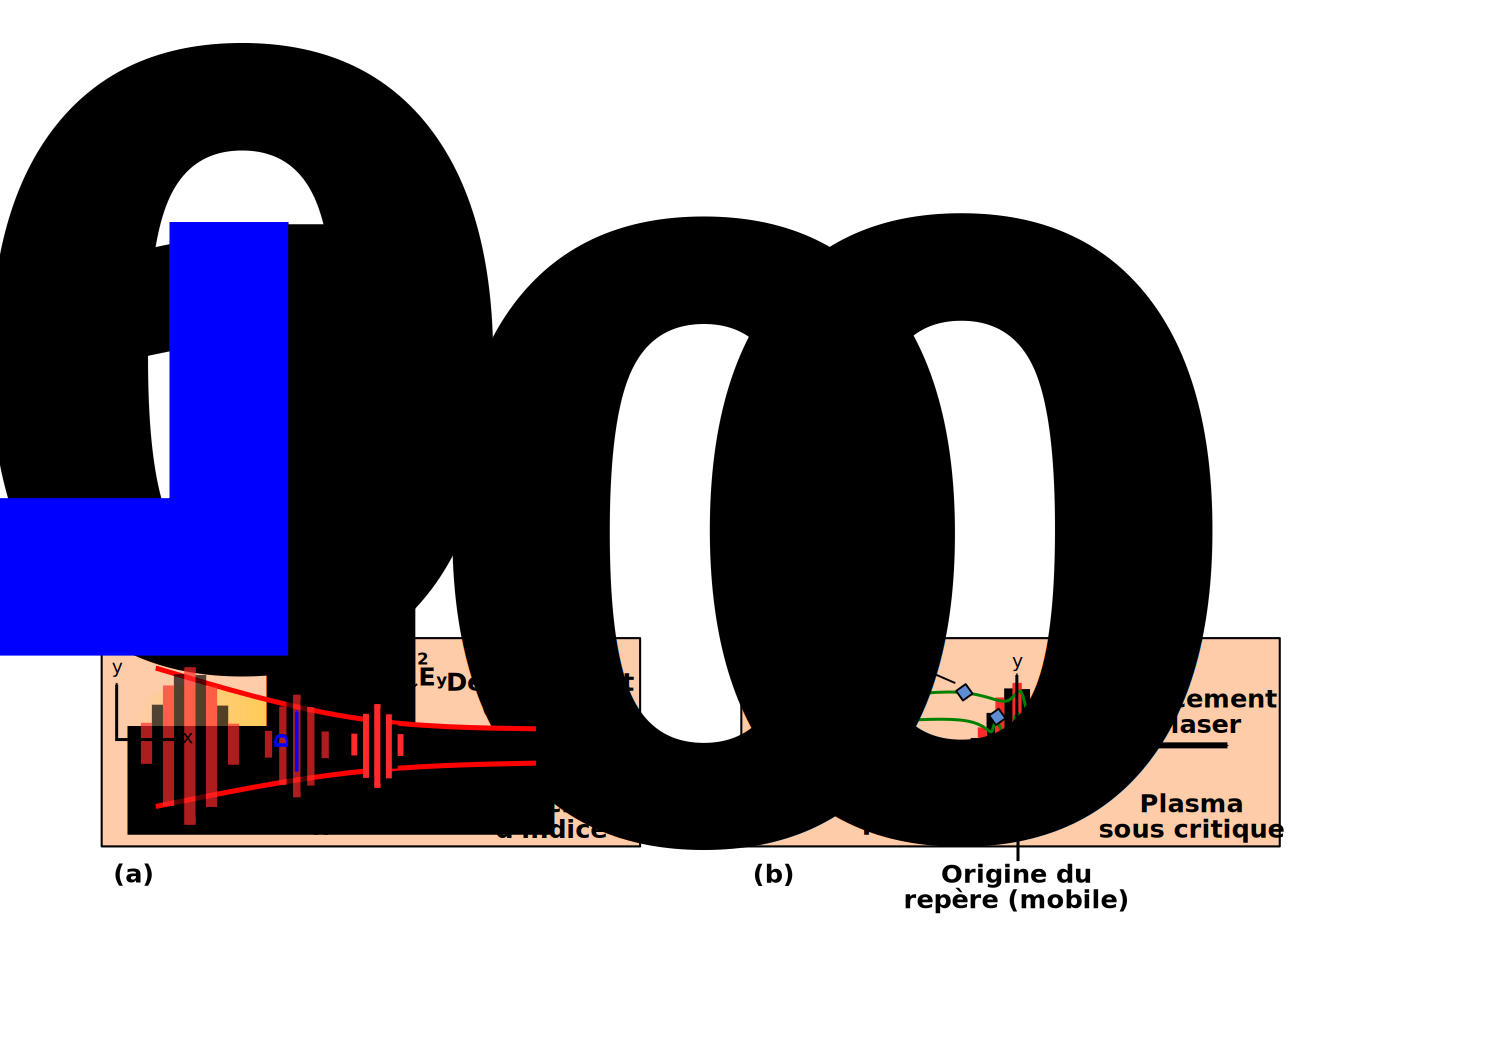
\includegraphics[width=\linewidth]{2-laser/interaction_laser_plasma.png}
    \caption{Illustration (a) de l'auto-focalisation relativiste et (b) de la force pondéromotrice dans un plasma sous-critique. Dans la figure (a) le laser se propage de gauche à droite dans un plasma sous-critique d'indice de réfraction $n_1$ alors que l'indice du plasma alentour est $n_0<n_1$. 
    Dans la figure (b) le repère est mobile et suit l'impulsion laser ; les particules défilent donc de droite à gauche dans la direction $-x$, et leur trajectoire est dessinée en vert. On 
    }
    \label{fig:2-interaction_laser_plasma}
\end{figure}

Ainsi, dans certaines conditions, une \textbf{zone de sous-densité électronique} peut donc être produite par le passage du laser. En particulier, un \textbf{canal sous-dense en électrons} peut être produit pour des intensités dépassant \parencite{gibbon_2013} : 
\begin{equation}
    I_0 > I_{canal} \approx 5.5\times 10^{19} ~ \dfrac{(D_L \si{[\um]})^2}{(\lambda_L \si{[\um]})^4} \dfrac{n_e}{n_c} ~ \si{[\W\per\cm^2]} ~ \rm .
    \label{eq:2-seuil_canal_ponderomoteur}
\end{equation}

Enfin, en plus des effets non-linéaires et relativistes présents pour des impulsions intenses d'extension spatiale limitée, des \textbf{effets de l'électrodynamique quantique en champ fort} peuvent aussi jouer un rôle important dès lors que la valeur du \textbf{paramètre quantique de l'électron} $\chi_e$ excède $\chi_e \gtrsim 0.1$ \parencite{zhang_2020}, avec \parencite{martinez_phd} :
\begin{equation}
    \chi_e = \dfrac{\gamma_e}{E_S} \sqrt{-\dfrac{\vec{E}_\parallel^2}{\gamma_e^2}+(\vec{E}_\perp + \vec{v} \times \vec{B})^2} ~ \rm ,
    \label{eq:2-chie_definition}
\end{equation}
où $E_S=m_e^2 c^3/e \hbar \approx 1.3 \times 10^{18} ~ \si{\V\per\m}$ est le champ de Sauter-Schwinger (aussi appelé simplement champ de Schwinger), qui est un champ caractéristique de l'électrodynamique quantique, et où $\vec{E}_\parallel$ et $\vec{E}_\perp$ sont respectivement les composantes parallèle et perpendiculaire du champ électrique par rapport à la vitesse $\vec{v}$ de l'électron. Ce paramètre est un invariant relativiste qui peut être compris comme étant le \textbf{champ électrique ressenti par la particule dans son référentiel propre}, normalisé à $E_S$ \parencite{dipiazza_2012}. Pour un électron relativiste oscillant dans une onde plane polarisée linéairement ($\gamma_e \sim \sqrt{1+a_0^2/2} \gg 1$ et $|\vec{E}_\perp+\vec{v} \times \vec{B}| \sim 2 \omega_L m_e c a_0/e$), on peut estimer que les effets de l'électrodynamique quantique doivent être considérés ($\chi_e \gtrsim 0.1$) dès lors que la valeur de $a_0$ est typiquement $a_0 \gtrsim 170$, ou encore $I_0 \gtrsim 4 \times 10^{22} ~ \si{\W \per \cm^2}$ (on a supposé une longueur d'onde de 1 µm). C'est aussi l'ordre de grandeur souvent considéré par les travaux théoriques pour inclure ces effets dans la description de \textbf{l'interaction laser-plasma} \parencite{dipiazza_2012, zhang_2020, capdessus_phd, martinez_phd}. 

Parmi les effets d'électrodynamique quantique en champ fort les plus notables (déjà évoqués au chapitre \ref{chap:1-particules}), nous pouvons mentionner la \textbf{production de paires électron-positron} par le processus Breit-Wheeler multi-photon ($\gamma + n \omega \to e^- + e^+$) et par le processus Trident multi-photon ($e + n \omega \to e + e^- + e^+$), ainsi que la \textbf{production de rayonnement énergétique} par le processus Compton inverse multi-photon ($e^- + n \omega \to e^- + \gamma$) \parencite{dipiazza_2012}. Pour ce type d'intensité laser, l'étude des mécanismes de rétroaction entre les effets d'électrodynamique en champ fort et la dynamique du plasma est un sujet de recherche très actif \parencite{zhang_2020, capdessus_phd}. 
Il est néanmoins intéressant de mentionner que l'influence de l'émission des photons sur la dynamique des électrons peut être modélisée d'un point de vue purement \textbf{classique} (force de friction) dès lors que la perte d'énergie des électrons peut être décrite de façon \textbf{continue} \parencite{burton_2014, niel_2018}. Des effets quantiques dans l'émission de rayonnement ont été mis en évidence par deux équipes en 2018 \parencite{poder_2018, cole_2018a} par la collision frontale d'un faisceau d'électrons d'énergie $>500 ~ \si{\MeV}$ avec un laser intense de $a_0 \gtrsim 10$. Cette configuration expérimentale permet en effet d'atteindre des valeurs de paramètre quantique $\chi_e$ significatives avec un laser d'intensité plus modérée (typiquement dès quelques $10^{21} ~ \si{\W\per\cm^2}$ pour un faisceau d'électrons d'énergie de l'ordre du $\si{\GeV}$ \parencite{vranic_2014}), et est à ce titre très étudiée dans le cadre d'études d'électrodynamique quantique en champ fort \parencite{vranic_2014, dipiazza_2012, zhang_2020}. 

Les différents régimes d'interaction laser-plasma évoqués jusqu'à présent sont résumés en figure \ref{fig:2-regimes_plasma}. L'axe des ordonnées indique l'intensité crête du laser considéré (de longueur d'onde 1 µm et de diamètre typique de tâche focale 10 µm), et l'axe des abscisses indique la densité électronique. Pour des intensités $\gtrsim 10^{18} ~ \si{\W \per \cm^2}$, les effets relativistes sont non négligeables $a_0 \gtrsim 1$, et deviennent de plus en plus importants à mesure que l'intensité augmente. Les effets d'électrodynamique quantique commencent aussi à être non négligeables dans l'interaction laser-plasma pour des intensités $\gtrsim 10^{22} ~ \si{\W \per \cm^2}$. Le seuil de transparence relativiste est indiqué par la ligne rouge, et est calculé via l'équation (\ref{eq:2-densite_critique_relativiste}). Les densités électroniques de quelques matériaux sont aussi indiquées à titre indicatif pour les conditions normales (ou ambiantes) de pression et de température (CNTP). La zone transparente au laser est indiquée par la zone 1. La force pondéromotrice y est toujours présente, et peut créer un canal sous-dense en électron en zones 1b et 1c (équation (\ref{eq:2-seuil_canal_ponderomoteur})). Le phénomène d'auto-focalisation relativiste est a priori significatif en zones 1c et 1d (équation (\ref{eq:2-seuil_auto-focalisation})). La zone 2 est opaque au rayonnement, et le laser pénètre seulement sur une épaisseur de peau. L'effet des collisions est d'autant plus important que la densité est importante, et que la température du plasma est faible, soit pour des intensités faibles. Les effets d'écrantage et d'oscillations plasma sont présents pour toutes les densités et intensités, ainsi que les phénomènes d'ionisation. D'autres processus non détaillés ici peuvent aussi intervenir dans l'interaction laser-plasma (voir figure \ref{fig:2-diversite_laser_fs}).

\begin{figure}[hbtp]
    \centering
    \includegraphics[width=0.8\linewidth]{2-laser/laser_plasma_zones.png}
    \caption{Résumé des différents régimes de propagation du laser dans l'interaction laser-plasma relativiste. En zone 1 le laser se propage dans le plasma, et peut créer un canal de sous-densité électronique en 1b et 1c, et être auto-focalisé en zones 1c et 1d. Il est réfléchi et pénètre seulement sur une épaisseur de peau en zone 2. Les paramètres quantifiant les effets de la relativité restreinte et de l'électrodynamique quantique (QED) sont aussi indiqués. Cette figure est disponible au format svg à l'adresse \url{github.com/lesnat/these} sous licence CC-BY et peut être librement adaptée.}
    \label{fig:2-regimes_plasma}
\end{figure}

En plus de ses effets sur la matière, l'interaction d'un laser intense avec un plasma peut aussi produire des particules énergétiques, en particulier des électrons et des photons $\gamma$.

\section{Production de particules énergétiques par laser}

Dans cette section, nous discuterons de l'utilisation de lasers intenses pour produire ou accélérer des particules de manière \textbf{directionnelle}, avec des énergies de \textbf{plusieurs MeV}.

Nous verrons en premier lieu comment utiliser astucieusement les propriétés des plasmas pour accélérer des \textbf{électrons}, en nous intéressant particulièrement aux processus d'accélérations dits d'\textit{accélération par sillage}, d'\textit{accélération directe} et d'\textit{accélération par $\vec{v} \times \vec{B}$}, respectivement importants dans les régimes sous-critiques, quasi-critiques et sur-critiques. D'autres mécanismes permettent néanmoins d'accélérer des électrons, ou de manière générale de transférer de l'énergie de l'impulsion laser au plasma, mais tous ne seront pas détaillés ici du fait de leur moins grande importance pour la suite de ce manuscrit. Certains de ces processus seront tout de même rapidement évoqués. De plus, nous ne discuterons ici que de l'accélération par un champ électromagnétique \textbf{laser}, et nous n'évoquerons donc pas les autres façons de produire des électrons énergétiques, tels que les méthodes utilisées dans les accélérateurs de particules, ou par la radioactivité $\beta^-$ par exemple.

Dans un second temps, nous verrons qu'en plus de leur potentiel pour l'accélération d'électrons, les lasers intenses constituent des candidats crédibles pour la production de \textbf{sources secondaires} tels que les \textbf{photons $\gamma$}. Nous verrons que ces lasers pourront être utilisés soit comme une source de \textbf{photons de basse énergie}, comme une source de \textbf{champ intense}, ou encore comme une façon de produire des \textbf{électrons énergétiques} qui seront ensuite utilisés pour la génération de particules secondaires. Nous présenterons enfin quatre schémas expérimentaux permettant de produire des sources de photons d'énergies autour du MeV par laser.


\subsection{Mécanismes d'accélération d'électrons}

Dans cette section, nous commencerons par étudier rapidement l'accélération par une onde plane d'un électron au repos dans le vide. Nous verrons notamment que, dans ces conditions, il n'est pas possible de lui transférer de l'énergie de manière permanente. Les sections suivantes présentent alors différentes méthodes permettant de contourner ce problème.

\subsubsection{Principe}

Pour comprendre l'interaction d'une onde électromagnétique avec des électrons dans un plasma, il peut être utile de commencer par considérer le cas théorique d'un seul électron dans le vide, interagissant avec une onde plane polarisée linéairement suivant $\vec{e}_y$ et se propageant dans la direction $\vec{e}_x$. Le potentiel vecteur de cette onde est : 
\begin{equation}
    \vec{A}(\xi)=A_0 \cos\left(\xi\right) ~ \vec{e}_y ~ \rm ,
\end{equation}
où $A_0$ est son amplitude maximale, et où $\xi=\dfrac{2 \pi}{\lambda_L} (x-ct)$ est sa phase. Pour un électron \textbf{initialement au repos à l'origine des positions}, on peut montrer \parencite{macchi_2012, yang_2011} que son impulsion est : 
\begin{equation}
    p_x=\dfrac{1}{4 m_e c} \left(\dfrac{e A_0}{c}\right)^2 \big[1+\cos(2 \xi)\big] ~ ; ~     p_y=\dfrac{e A_0}{c}\sin(\xi) ~ ; ~ p_z=0 \rm .
\end{equation}

Le déplacement de l'électron est alors contenu dans le plan $(\vec{e}_x,\vec{e}_y)$, et on peut remarquer que le \textbf{mouvement transverse} de l'électron est \textbf{oscillant à la même phase que l'onde}. Cette composante est directement proportionnelle à l'intensité du champ, et est donc significative sur le mouvement de l'électron (initialement au repos) \textbf{même pour des intensités faibles}. La composante \textbf{longitudinale} de l'impulsion de l'électron peut quant à elle être exprimée comme une \textbf{somme de deux termes} :
\begin{itemize}
    \item un terme proportionnel à $\cos(2 \xi)$ oscillant à \textbf{2 fois} la phase de l'onde, et 
    \item un terme $\dfrac{1}{4 m_e c} \left(\dfrac{e A_0}{c}\right)^2$ qui \textbf{ne dépend pas de la phase}, et correspond donc à un \textbf{mouvement de dérive constant} de l'électron dans la direction de $\vec{e}_x$.
\end{itemize}

Cette composante longitudinale est influencée seulement par le \textbf{champ magnétique} de l'onde, car la composante électrique de la force de Lorentz ne permet pas d'accélérer l'électron selon cette direction. Dans ce cas, l'impulsion \textbf{longitudinale} est proportionnelle au \textbf{carré} de l'amplitude de l'onde, et est donc \textbf{négligeable pour des intensités faibles} ($a_0\ll 1$, avec $a_0=e A_0/m_e c$), et \textbf{importante pour des intensités fortes} ($a_0 \gtrsim 1$). De plus, une fois que le mouvement de dérive a été initié, chaque phase accélératrice est suivie d'une phase décélératrice, et la \textbf{moyenne} du mouvement de l'électron sur \textbf{un cycle} donne donc au final un \textbf{gain d'énergie total nul}. 

Ce dernier aspect peut être généralisé, et est alors appelé \textbf{théorème de Lawson-Woodward}. Celui-ci stipule qu'il est impossible de transférer de l'énergie d'une onde plane à un électron dans le vide \textbf{de manière permanente} \parencite{esarey_2009, zaim_phd, gibbon_2013}, sous certaines hypothèses qui peuvent être résumées par \parencite{esarey_2009} :
\begin{enumerate}
\def\labelenumi{\arabic{enumi}.}
    \item la région d'interaction est supposée infinie,
    \item le laser se propage dans le vide sans murs ni bords,
    \item l'électron est ultra-relativiste dans la direction d'accélération,
    \item aucun champ électrique ou magnétique externe ne sont présents, et
    \item les effets non linéaires (force pondéromotrice, freinage par rayonnement, ...) sont négligés.
\end{enumerate}

Tout mécanisme d'accélération d'électrons par laser se devra alors d'\textbf{invalider au moins une de ces hypothèses} pour pouvoir produire un \textbf{gain net d'énergie} des électrons. 
Dans la suite, nous présenterons alors certains de ces mécanismes, même si nous ne rentrerons pas dans le détail de leur modélisation physique.

\subsubsection{Cible sous-critique et accélération par sillage}

Commençons tout d'abord par discuter de l'accélération d'électrons lors de la propagation d'un laser dans un plasma \textbf{sous-critique}, qui est très étudiée depuis la fin des années 1970 \parencite{tajima_1979}. Plusieurs régimes physiques d'accélération d'électrons ont été proposés (une revue est disponible en référence \parencite{esarey_2009}), mais nous discuterons ici particulièrement du mécanisme d'\textbf{accélération par sillage} (\textit{Laser Wakefield acceleration} en anglais), et principalement du \textbf{régime de la bulle} (\textit{blowout regime}). Celui-ci a été découvert théoriquement en 2002 \parencite{pukhov_2002} et a été mis en évidence expérimentalement 2 ans plus tard par trois équipes différentes \parencite{faure_2004, geddes_2004, mangles_2004}. Il est alors très étudié depuis, puisqu'il permet de produire des faisceaux d'électrons d'une \textbf{grande qualité} (par rapport aux autres modes d'accélération par laser), notamment de par leur \textbf{distribution en énergie très piquée}, avec une largeur de bande de typiquement quelques \%, et une \textbf{divergence angulaire faible}, typiquement quelques dixièmes de milliradians \parencite{esarey_2009}. De plus, l'\textbf{énergie} cinétique des électrons accélérés \textbf{peut être contrôlée} par un choix judicieux de paramètres laser-plasma, et atteindre des valeurs \textbf{de quelques MeV à plusieurs GeV} \parencite{faure_2019, leemans_2006, gonsalves_2019}. Enfin, le milieu utilisé pour l'accélération d'électrons étant typiquement un jet de gaz, la cible peut se renouveler continûment, permettant (en principe) de produire de tels faisceaux de particules avec un \textbf{haut taux de répétition}. Pour notre application, une de leurs limitations majeures par rapport à d'autres modes d'accélération concerne néanmoins la \textbf{charge totale du faisceau} d'électrons, qui est typiquement limitée à \textbf{quelques centaines de pico-Coulombs}. D'autres mécanismes d'accélération par laser dans un plasma sous dense peuvent quant à eux produire des faisceaux de quelques nanocoulombs, mais avec des propriétés nettement moins intéressantes en terme de dispersion angulaire et énergétique \parencite{esarey_2009}. 

Dans ce régime d'accélération, une impulsion laser d'\textbf{intensité relativiste} ($a_0 \gtrsim 1$) se propage dans un plasma \textbf{sous-critique}. Par l'intermédiaire de sa \textbf{force pondéromotrice}, elle peut éjecter les électrons sur son passage et créer une \textbf{cavité}, ou \textbf{bulle} quasiment \textbf{vide d'électrons} dans son sillage \parencite{pukhov_2002}. La \textbf{séparation de charge} produite induit ainsi un fort \textbf{champ électrique longitudinal}, qui peut \textbf{accélérer des électrons dans la direction de propagation du laser} si ceux-ci ont été convenablement injectés dans la cavité \parencite{pukhov_2002, esarey_2009}. Ce mécanisme est illustré schématiquement en figure \ref{fig:2-acceleration_sillage}. Les électrons les plus accélérés par ce champ sont alors ceux qui restent le plus longtemps \textbf{en phase} avec le champ accélérateur. Plusieurs mécanismes peuvent néanmoins limiter leur gain d'énergie maximal, que ce soit la diffraction de l'impulsion laser, le déphasage des électrons et du champ accélérateur, la perte d'énergie du laser au fur et à mesure de sa propagation, ou encore des instabilités laser-plasma \parencite{esarey_2009}.

\begin{figure}[hbtp]
    \centering
    \includegraphics[width=0.7\linewidth]{2-laser/acceleration_sillage_bulle.png}
    \caption{Illustration du mécanisme d'accélération par sillage dans le régime de la bulle. La force pondéromotrice de l'impulsion laser créé une cavité sous-dense en électrons dans son sillage, ce qui a pour effet de produire un champ électrique longitudinal. Les électrons injectés dans la cavité peuvent alors être accélérés dans la direction de propagation du laser.}
    \label{fig:2-acceleration_sillage}
\end{figure}

Pour créer une cavité sous dense en électrons de façon efficace, l'extension spatiale du laser doit être typiquement de l'ordre de grandeur de la longueur d'onde des oscillations plasma, et la force pondéromotrice doit pouvoir équilibrer le champ de rappel produit par le défaut de charges, ce qui peut se traduire par les conditions \parencite{esarey_2009, gordienko_2005} :
\begin{equation}
    c \tau_L \lesssim D_L ~ ; ~ \dfrac{\omega_{pe}}{c} D_L \sim \sqrt{a_0} ~ \rm .
    \label{eq:2-parametres_bulle}
\end{equation}

En pratique, les valeurs de $a_0$ considérées dans ce régime sont souvent de l'ordre de quelques unités \parencite{esarey_2009, faure_2019}. Les lasers de \textbf{haute puissance} (plusieurs centaines de TW) sont alors en pratique \textbf{peu focalisés} dans des matériaux \textbf{peu denses}, et, leur longueur de Rayleigh étant dans ce cas importante, ils peuvent \textbf{accélérer des électrons sur de grandes distances}, jusqu'à des \textbf{énergies très importantes} (par exemple jusqu'à 8 GeV pour un laser de 850 TW focalisé sur un diamètre de 70 µm pendant environ 20 cm à l'aide de capillaires \parencite{gonsalves_2019}). Au contraire, les lasers de \textbf{faible puissance} sont \textbf{plus focalisés} dans des matériaux plus \textbf{denses}, et accélèrent des particules \textbf{de plus faibles énergies sur de plus courtes distances} (par exemple un laser de 1 TW focalisé sur un diamètre de 2 µm pendant une distance 25 µm produit des électrons autour de 10 MeV \parencite{faure_2019}). Néanmoins, cette discussion qualitative ne résume pas la complexité du sujet, où la longueur d'accélération et la densité de la cible doivent aussi être choisis pour \textbf{optimiser la phase relative des électrons et de l'onde plasma}, et où l'injection des électrons dans la bulle constitue un enjeu de taille \parencite{esarey_2009}. 

Dans un cas satisfaisant les propriétés de l'équation \ref{eq:2-parametres_bulle}, il est possible d'estimer l'énergie cinétique $E_e^{bulle}$ des électrons accélérés, ainsi que leur nombre $N_e^{bulle}$ via \parencite{gordienko_2005} :
\begin{equation}
    E_e^{bulle} \si{[\MeV]}\sim ~ 1.1 ~ \dfrac{\tau_L \si{[\fs]}}{\lambda_L\si{[\um]}} \sqrt{P_0\si{[\TW]}} ~ ; ~ N_e^{bulle} \sim ~ 1.1 \times 10^9 ~ \lambda_L\si{[\um]} \sqrt{P_0\si{[\TW]}}\rm .
    \label{eq:2-scaling_Gordienko}
\end{equation}

Les énergies et nombres d'électrons typiquement atteignables par accélération par sillage dans le régime de la bulle sont alors tracés en figure \ref{fig:2-scaling_Gordienko}, pour les gammes de puissances et d'énergie pertinentes dans notre cas, et pour une longueur d'onde $\lambda_L=1 ~ \si{\um}$.

\begin{figure}[hbtp]
    \centering
    \includegraphics[width=0.7\linewidth]{2-laser/scaling_Gordienko.png}
    \caption{Estimations de l'énergie typique des électrons accélérés par sillage dans le régime de la bulle (graphique supérieur) ainsi que leur nombre (graphique inférieur), en fonction de la puissance laser. La charge totale est aussi indiquée en nanocoulombs (nC).}
    \label{fig:2-scaling_Gordienko}
\end{figure}

Comme évoqué précédemment, les énergies typiques sont de l'ordre de la centaine de MeV, et la charge totale du faisceau ne dépasse pas quelques nanocoulombs. Ces valeurs sont néanmoins seulement des \textbf{estimations}, et plusieurs techniques permettent de significativement modifier ce régime d'interaction. Il a par exemple été démontré que la génération d'énergies de l'ordre du \textbf{GeV} est possible avec seulement \textbf{40 TW} de puissance \parencite{leemans_2006} en utilisant des capillaires pour le guidage de l'impulsion sur de très longues distances. Au contraire, des expériences récentes ont démontré la production de faisceaux d'énergie autour du MeV, de \textbf{quelques pC} en focalisant une impulsion de quelques TW dans des jets de gaz denses de quelques 10 µm d'épaisseurs, mais avec un \textbf{taux de répétition de l'ordre du kHz} \parencite{faure_2019}. Les valeurs de charge totale données par ce modèle semblent aussi assez optimistes.

\subsubsection{Cible quasi-critique et accélération directe}

Comme nous l'avons vu précédemment, lorsqu'un laser interagit avec un plasma \textbf{sous-critique} il peut se propager sur des distances importantes, et ainsi accélérer des particules \textbf{en volume}. Pour le mécanisme d'accélération par sillage dans le régime de la bulle, l'impulsion laser doit rester suffisamment stable sur toute sa distance de propagation pour accélérer des particules de façon efficace, et une part non négligeable de son énergie n'est donc pas transférée aux particules.
Au contraire, pour un matériau de densité proche de la densité critique relativiste, appelé \textbf{quasi-critique}, le laser peut être significativement altéré lors de son interaction avec le plasma, et potentiellement y transférer une part plus importante de son énergie \parencite{gahn_1999a}. 
Parmi ces effets d'absorption, nous pouvons mentionner ici le mécanisme d'\textbf{accélération directe}, qui permet de produire \textbf{un nombre important} de particules (actuellement observé jusqu'à presque 100 nC de charge totale \parencite{ma_2018}) avec une \textbf{distribution en énergie large} pouvant atteindre \textbf{plusieurs centaines de MeV} \parencite{pukhov_1999}. 
Ce mécanisme a été décrit théoriquement dès la fin des années 1990 \parencite{pukhov_1999}, et il est notamment supposé jouer un rôle important pour l'accélération d'électrons dans les \textbf{long pré-plasma} lors de l'interaction laser-solide \parencite{pukhov_1999, krygier_2014}. 
Dans ce contexte, il est donc en compétition avec d'autres mécanismes d'accélération présents aux différentes densités du pré-plasma. Plusieurs expériences attribuent néanmoins des résultats de mesure à l'accélération directe dans des jets de gaz denses avec des durées d'impulsions de quelques centaines de fs \parencite{gahn_1999a, mangles_2005a}. Son étude est toujours active, par l'intermédiaire de modèles théoriques, de simulations numériques ou d'expériences \parencite{arefiev_2016, jirka_2020, krygier_2014, thevenet_2016}.

Comme nous l'avons vu précédemment, l'accélération d'électrons à partir d'une onde plane n'est pas possible \textbf{dans le vide}, car l'énergie gagnée par l'électron dans une phase accélératrice est ensuite perdue dans une phase décélératrice. 
Dans le mécanisme d'\textbf{accélération directe}, des \textbf{champs électromagnétiques externes} vont permettre à l'électron de \textbf{rester plus longtemps dans la phase accélératrice}, et ainsi pouvoir atteindre une énergie \textbf{plusieurs fois supérieures à l'énergie atteignable dans le vide} \parencite{arefiev_2016, jirka_2020, krygier_2014}.
En particulier, la présence d'un champ \textbf{transverse} à la direction de propagation du laser peut sous certaines conditions (fréquence du laser de l'ordre de la fréquence bétatron \parencite{corde_2013a}) faire osciller des électrons dans un mouvement appelé \textbf{bétatron} \parencite{pukhov_1999}, et ainsi \textbf{légèrement les déphaser} par rapport au champ laser ; leur permettant de rester en phase accélératrice plus longtemps que si ce champ transverse n'était pas présent.
En pratique, ces champs peuvent être produits directement par le laser, via le creusement d'un \textbf{canal sous-dense en électron} dans le plasma par la force pondéromotrice (voir section précédente). 
Cette \textbf{séparation de charges} produit en effet un champ électrique \textbf{transverse}, ainsi qu'un champ électrique longitudinal à l'interface vide-plasma \parencite{arefiev_2016}, et le courant d'électrons accélérés peut aussi induire un champ magnétique azimutal \parencite{jirka_2020, arefiev_2016}. L'effet croisé de ces champs induits et du champ laser peut alors rendre la trajectoire de l'électron très complexe, lui permettant parfois de rester en phase accélératrice pendant de longues distances, et parfois non.
Ce mécanisme d'accélération est ainsi extrêmement sensible aux conditions initiales d'injection des électrons \parencite{arefiev_2016, krygier_2014}.
Il est illustré très schématiquement en figure \ref{fig:2-acceleration_directe}, où la figure supérieure représente la trajectoire d'un électron accéléré par l'onde dans le vide, et la figure inférieure représente une trajectoire où l'effet global des champs a été bénéfique pour l'accélération, en déphasant l'électron par rapport à l'onde laser et lui permettant d'être accéléré plus longtemps.

\begin{figure}[hbtp]
    \centering
    \includegraphics[width=0.6\linewidth]{2-laser/acceleration_directe.png}
    \caption{Illustration du mécanisme d'accélération directe. En figure (a) l'électron a été accéléré dans le vide, sans gain d'énergie net après le passage du laser. En figure (b) la présence d'un champ électrique transverse créé par un canal sous-dense en électrons permet à l'électron de rester en phase accélératrice sur de longues distances, et donc d'acquérir une énergie cinétique importante.}
    \label{fig:2-acceleration_directe}
\end{figure}

Pour que ce mécanisme puisse avoir lieu dans un plasma quasi-critique homogène, la condition pour la production d'un canal sous dense en électrons par force pondéromotrice (équation (\ref{eq:2-seuil_canal_ponderomoteur})) doit être satisfaite, et il est aussi possible de montrer \parencite{arefiev_2016} que le seuil à partir duquel le phénomène de gain par oscillations bétatron transverses commence à devenir important est :
\begin{equation}
    G_{AD} =a_0 \sqrt{\dfrac{n_e}{n_c}} > 1 ~ \rm .
\end{equation}

Pour l'accélération directe ayant lieu dans \textbf{un pré-plasma de profil de densité exponentiel}, on peut approximer la forme de la distribution en énergie des électrons par une fonction exponentielle décroissante $f(E_e) \propto \exp(-E_e/T_e^{AD})$, avec $T_e^{AD}$ une énergie caractéristique souvent appelée \textit{température effective} qui peut être estimée comme \parencite{pukhov_1999} :
\begin{equation}
    T_e^{AD} \si{[\MeV]}\sim 1.5 \times 10^{-9} \sqrt{I_0 \si{[\W\per\cm^2]}} ~ \rm .
\end{equation}

Pour ce type de distributions en énergie, l'énergie totale contenue dans ces électrons est de l'ordre de $N_e^{AD} ~ T_e^{AD}$, et on peut donc estimer leur nombre total via :
\begin{equation}
    N_e^{AD} \sim 6.3 \times 10^{12} ~ \dfrac{\eta_{L \to e}^{AD} ~ E_L \si{[J]}}{T_e^{AD} \si{[MeV]}} ~ \rm ,
    \label{eq:2-acceleration_directe_nombre}
\end{equation}
où $\eta_{L \to e}^{AD}$ est l'efficacité d'absorption du laser dans ces électrons, qui peut varier de \textbf{quelques \%} si on considère seulement les électrons \textbf{éjectés}, à \textbf{plusieurs dizaines de \%} si on considère tous les électrons \textbf{accélérés} \parencite{pukhov_1999}. Des valeurs typiques de température effective et de nombre sont alors représentées en figure \ref{fig:2-scaling_acceleration_directe} en fonction de la puissance laser, où on a considéré une absorption de 30\%, une tache focale de largeur à mi-hauteur $10 ~ \si{\um}$ et une durée d'impulsion de largeur à mi-hauteur $30 ~ \si{\fs}$.

\begin{figure}[hbtp]
    \centering
    \includegraphics[width=0.7\linewidth]{2-laser/scaling_Pukhov.png}
    \caption{Estimations de la température effective et du nombre d'électrons accélérés par accélération directe dans un pré-plasma long, en fonction de la puissance laser.}
    \label{fig:2-scaling_acceleration_directe}
\end{figure}

Ces estimations montrent donc que ce type de situations permet d'atteindre des \textbf{températures effectives de plusieurs dizaines de MeV}, et des charges typiques de \textbf{dizaines de nanocoulombs} (jusqu'à 100 nC ont été observés et \textbf{attribués au mécanisme d'accélération directe} pour un laser de 200 TW, avec une durée d'interaction de l'ordre de 700 fs et 150J d'énergie laser \parencite{ma_2018}). Celles-ci reposent néanmoins sur des simplifications très importantes de la physique de l'interaction laser-plasma, qui peut s'avérer très complexe dans ce type de régimes, et ne doivent donc pas être prises comme des estimations trop quantitatives.

En effet, de nombreux autres mécanismes peuvent aussi entrer en jeu lors de l'interaction de ce type de laser avec un plasma de densité quasi-critique, tels que des instabilités paramétriques, qui permettent de transférer une part de l'énergie de l'onde laser à des ondes plasma. Ce type d'instabilités ne sera néanmoins pas présenté car sortant du cadre de cette thèse, mais plus d'informations sont disponibles notamment dans les références \parencite{moreau_phd, kruer_2003}. La fabrication de cibles de densité quasi-critique, permettant notamment d'étudier ce régime plus finement d'un point de vue expérimental, est aussi aujourd'hui un enjeu important \parencite{passoni_2020, prencipe_2017}.

\subsubsection{Cible sur-critique et accélération $\vec{v} \times \vec{B}$}

Pour des plasmas encore plus denses que ceux évoqués précédemment, la propagation du laser n'est plus possible. L'interaction d'un laser avec un matériau sur-critique (typiquement un solide ou un liquide) se fera alors non plus en volume mais seulement en \textbf{surface}, ou plus rigoureusement sur une profondeur limitée à l'épaisseur de peau. Les sources d'électrons produits par ce type d'interactions ont une \textbf{distribution en énergie large}, typiquement de forme \textbf{exponentielle décroissante} \parencite{malka_1996}, et une divergence angulaire de plusieurs dizaines de degrés de demi-angle \parencite{debayle_2010}. Ce type de régime d'interaction permet aussi de produire des \textbf{courants d'électrons très importants} à l'intérieur du solide \parencite{macchi_2012}. Nous discuterons ici en particulier du mécanisme d'accélération par la composante magnétique de la force de Lorentz, aussi noté $\vec{v} \times \vec{B}$ ou $\vec{J} \times \vec{B}$, qui peut être significatif dès lors que l'effet du champ magnétique devient important, i.e. pour des intensités relativistes $a_0 \gtrsim 1$. 

Comme nous avons pu le voir au début de cette section, lors de l'interaction d'une onde plane avec un électron initialement au repos dans le vide, ce dernier peut être accéléré notamment par la composante électrique du champ laser et acquérir une vitesse transverse à la direction de propagation de l'onde. Si le champ magnétique est suffisamment intense, le terme magnétique de la force de Lorentz peut faire osciller cet électron \textbf{longitudinalement}. L'énergie cinétique accumulée par cette particule lors de la phase accélératrice est néanmoins perdue lors d'une phase décélératrice. Dans le mécanisme d'accélération appelé $\vec{v} \times \vec{B}$, le laser se situe au niveau d'une \textbf{interface sur-critique}, et le mouvement d'\textbf{oscillation longitudinal} des électrons est alors \textbf{interrompu} lors du passage de l'interface sur-critique. Les électrons injectés dans la cible en ayant une vitesse longitudinale ne peuvent en effet plus être décélérés par l'onde électromagnétique, qui est évanescente derrière l'interface sur-critique, et ceux-ci conservent donc une part de l'énergie cinétique qu'ils ont acquise en phase accélératrice. Ce principe est illustré en figure \ref{fig:2-acceleration_magnetique}c. 
Dans l'interaction laser-solide, le nombre d'électrons injectés peut être très important (avec une densité de courant de l'ordre de $\sim e ~ n_c ~ c$ \parencite{macchi_2012}), ce qui créé une séparation de charges à l'interface sur-critique. Le champ électrostatique induit par cette séparation de charge a alors tendance à \textbf{freiner les électrons injectés} dans le matériau, jusqu'à pouvoir les arrêter totalement \parencite{macchi_2012}. En pratique, ce défaut de charges est \textbf{spontanément compensé} par un \textbf{courant de retour} d'électrons thermiques peu énergétiques, souvent appelés \textit{électrons froids}, qui a tendance à \textbf{neutraliser les charges et les courants} \parencite{macchi_2012, bell_1997}. 
Les électrons les plus énergétiques (chauds et suprathermiques) peuvent ainsi se propager dans le solide, en étant toutefois freinés par le champ électrostatique de séparation de charges \parencite{macchi_2012, bell_1997}.

\begin{figure}[hbtp]
    \centering
    \includegraphics[width=0.7\linewidth]{2-laser/acceleration_magnetique.png}
    \caption{Principe de l'accélération par $\vec{v} \times \vec{B}$. En (a) le laser accélère l'électron dans le plasma, qui acquiert une vitesse longitudinale par l'effet de la force magnétique. Il ne peut cependant pas obtenir de gain permanent en énergie car chaque phase accélératrice est suivie d'une phase décélératrice. En (b) une interface sur-critique permet à l'électron de conserver son énergie, car il est injecté dans la cible avant d'avoir pu être totalement décéléré.}
    \label{fig:2-acceleration_magnetique}
\end{figure}

De nombreuses expériences et simulations numériques tendent à montrer que la distribution en énergie des électrons accélérés dans l'interaction laser-solide est typiquement exponentielle décroissante, de \textit{température effective} \parencite{macchi_2012} :
\begin{equation}
    T_e^{\vec{v} \times \vec{B}} \sim \left(\sqrt{1+a_0^2/2}-1\right) m_ec^2 ~ \rm . 
\end{equation}

En utilisant un raisonnement similaire à celui qui a été mené pour dériver l'équation (\ref{eq:2-acceleration_directe_nombre}), on peut aussi estimer le nombre total d'électrons accélérés comme étant :
\begin{equation}
    N_e^{\vec{v} \times \vec{B}} \sim 6.3 \times 10^{12} ~ \dfrac{\eta_{L \to e}^{\vec{v} \times \vec{B}} ~  E_L \si{[J]}}{T_e^{\vec{v} \times \vec{B}} \si{[MeV]}} ~ \rm ,
\end{equation}
où $\eta_{L\to e}$ est une estimation de l'absorption du laser par les électrons, que l'on peut prendre de l'ordre de 10\% \parencite{price_1995, malka_1996}. Les énergies et nombres d'électrons typiques produits par ce mécanisme sont illustrés en figure \ref{fig:2-scaling_ponderomoteur}, où on a supposé une durée d'impulsion laser de largeur à mi-hauteur $30 ~ \si{\fs}$, une tache focale de largeur à mi-hauteur $10 ~ \si{\um}$ et une longueur d'onde de $1 ~ \si{\um}$. 
\begin{figure}[hbtp]
    \centering
    \includegraphics[width=0.7\linewidth]{2-laser/scaling_ponderomoteur.png}
    \caption{Estimations de la température effective et du nombre d'électrons accélérés par $\vec{v} \times \vec{B}$ ($\vec{v} \times \vec{B}$) dans l'interaction laser-solide, en fonction de la puissance laser. On a considéré une tache focale laser de largeur à mi-hauteur 10 µm.}
    \label{fig:2-scaling_ponderomoteur}
\end{figure}

On observe donc que la température effective est ici typiquement de \textbf{quelques MeV à quelques dizaines de MeV} et que la charge totale est de l'ordre de \textbf{quelques dizaines de nanocoulombs}, ce qui semble être en accord avec des données expérimentales typiques de l'interaction laser-solide \parencite{malka_1996, dubois_2014}. Ces estimations reposent néanmoins ici aussi sur des simplifications très importantes de la physique de l'interaction laser-plasma, et ne remplacent donc pas des études plus approfondies (notamment par l'intermédiaire de simulations numériques).

Dans l'interaction laser-solide, le mécanisme $\vec{v} \times \vec{B}$ peut aussi être en concurrence avec d'autres mécanismes d'accélération d'électrons, comme par exemple le chauffage stochastique \parencite{bourdier_2005, chopineau_2019}, ou l'effet Brunel pour un laser en incidence oblique en polarisation p \parencite{brunel_1987, chopineau_2019}. D'un point de vue expérimental, les propriétés des électrons injectés dans une cible solide ne peuvent pas être mesurées de manière directe, et doivent être déduites de mesures indirectes ou des propriétés des électrons éjectés de la cible, qui peuvent avoir été significativement affectées lors de leur propagation (par des collisions ou des champs électrostatiques par exemple) \parencite{link_2011a}.

\subsubsection{Comparaison des différents régimes d'accélération}

Comme nous avons pu le voir dans les sections précédentes, l'interaction laser-plasma dans le régime relativiste peut faire intervenir de nombreux processus (dont plusieurs n'ont pas été abordés ici, voir figure \ref{fig:2-diversite_laser_fs}), et la propagation du laser dans le plasma est fortement influencée par son intensité, son extension spatio-temporelle, et la densité et température des électrons du plasma notamment. De plus, les mécanismes d'accélération d'électrons par laser font souvent intervenir une \textbf{combinaison} de ces processus en synergie (ionisation, transparence relativiste, force pondéromotrice, ...). Ainsi, l'utilisation de \textbf{certains} paramètres laser (intensité, extension spatio-temporelle, contraste, ...) avec \textbf{certains} paramètres de cible (densité, matériau, géométrie, épaisseur, ...) va \textbf{fortement influencer} l'apparition des différents mécanismes d'accélération d'électrons, leur efficacité respective, et enfin les caractéristiques principales des sources d'électrons obtenues (charge, forme de la distribution en énergie, énergie caractéristique, distribution angulaire, ...). 
Par exemple, les conditions optimales pour l'\textbf{accélération par sillage dans le régime de la bulle} se situent à \textbf{intensité modérée et densité faible}, tandis que l'accélération par \textbf{$\vec{v} \times \vec{B}$} nécessite une \textbf{densité sur-critique}, et produit des particules d'autant plus énergétiques que l'\textbf{intensité du laser est élevée}. L'\textbf{accélération directe} peut être importante lorsque \textbf{l'intensité et la densité sont suffisantes} pour produire un canal sous-dense. Les différents régimes d'accélération d'électrons par laser sont illustrés en figure \ref{fig:2-regimes_electron}. Il est important de noter que cette figure suppose une longueur d'onde laser de 1 µm et une tache focale de 10 µm, et que ces zones peuvent donc être significativement différentes pour d'autres paramètres laser. La zone 1 indique les paramètres optimaux pour l'accélération par sillage dans le régime de la bulle, qui correspond ici à un laser d'environ 10 TW (en fixant la valeur de $a_0$ et de la taille de la tache focale on peut en déduire les autres paramètres). Les densités optimales peuvent ici grandement varier en fonction des choix de paramètres laser-plasma considérés (des exemples sont donnés dans la référence \parencite{faure_2019}). La zone 2 correspond au régime d'accélération directe, caractérisé par un gain important par rapport à l'accélération dans le vide, et une intensité suffisante pour la formation d'un canal sous-dense. La zone 3 correspond grossièrement à la zone quasi-critique, où la propagation du laser dans le plasma est fortement perturbée, et où de nombreux effets de couplage laser-plasma entrent en ligne de compte. Cette zone est aussi importante dans l'interaction laser-solide, de par l'expansion du solide à des densités quasi-critiques après son chauffage par l'impulsion principale ou par une pré-impulsion (contrôlée ou non). La zone 4 correspond à l'interaction laser-solide, ou laser-liquide. En particulier, dans la zone 4b les effets de la force magnétique sont importants, alors que l'accélération d'électrons dans la zone 4a nécessite de faire intervenir d'autres mécanismes, tels que l'effet Brunel pour une incidence oblique en polarisation p. Cette figure peut bien entendu être superposée à la figure \ref{fig:2-effets_plasma} afin d'estimer quels effets sont susceptibles d'interagir lors d'un choix d'intensité ou de densité de plasma considéré. 

\begin{figure}[hbtp]
    \centering
    \includegraphics[width=0.8\linewidth]{2-laser/laser_electron_zones.png}
    \caption{Régimes d'accélération d'électrons par laser pour différentes intensités et densités de plasma, en considérant un laser typique de longueur d'onde 1 µm focalisé sur un diamètre typique de 10 µm. En zone 1 on considère l'accélération par sillage dans le régime de la bulle, tandis que la zone 2 correspond aux paramètres typiques de l'accélération directe. La zone 3 permet de regrouper les nombreux effets pouvant avoir lieu à une densité quasi-critique. La zone 4 indique les régimes d'accélération par effet Brunel en 4a et par force magnétique en 4b. Dans ce cas la zone 4a s'étend au delà de la limite $a_0 \gtrsim1$ tandis que la zone 4b est limitée aux intensités relativistes $a_0 \gtrsim 1$.}
    \label{fig:2-regimes_electron}
\end{figure}

En pratique, il est aussi possible de choisir des schémas expérimentaux (géométries de cibles, intensité laser, ...) qui peuvent \textbf{combiner} différents régimes d'accélération. On peut par exemple citer l'utilisation en synergie des mécanismes d'accélération directe et d'accélération par sillage \parencite{zhang_2015b}, ou de l'accélération directe combinée à l'accélération par $\vec{v} \times \vec{B}$ par exemple \parencite{krygier_2014, pazzaglia_2020, jiang_2014}. Compte tenu de la physique très riche de ces régimes d'interaction, il est donc souvent nécessaire d'avoir recours à des \textbf{simulations numériques} pour pouvoir estimer les propriétés des sources d'électrons.

\subsection{Production de photons gamma par laser}

Dans cette section, nous discuterons particulièrement de différentes manières de produire des photons d'énergies multi-MeV par laser. Comme nous l'avons évoqué au début de ce chapitre, les lasers peuvent être à la fois vu comme une source de photons de basse énergie, ou comme une source de champ électromagnétique intense, et permettent de plus de produire des électrons énergétiques. Nous verrons que ces trois aspects pourront être mis à profits pour la production de photons de plusieurs MeV. Nous discuterons particulièrement ici des processus Compton inverse linéaire, Compton (ou Thomson) inverse multi-photon et Bremsstrahlung, tels que décrits dans le chapitre \ref{chap:1-particules}. Nous présenterons ici quatre configurations expérimentales spécifiques, que sont la collision frontale (ou contra-propagative) d'un faisceau d'électrons avec un laser peu intense (production de photons via le processus Compton inverse linéaire), la collision frontale d'un faisceau d'électrons avec un laser intense (production de photons via le processus Compton inverse multi-photon), la co-propagation d'un laser intense avec un faisceau d'électrons qu'il a lui même accéléré (production de photons via le processus Compton inverse multi-photon), et l'injection d'un faisceau d'électrons (qui peut avoir été produit par laser) dans un matériau solide appelé convertisseur (production de photons via le processus Bremsstrahlung). Ces diverses configurations sont illustrées en figure \ref{fig:2-config_gamma_laser}a, \ref{fig:2-config_gamma_laser}b, \ref{fig:2-config_gamma_laser}c et \ref{fig:2-config_gamma_laser}d, respectivement.

\begin{figure}[hbtp]
    \centering
    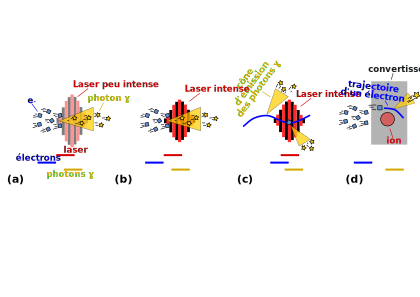
\includegraphics[width=\linewidth]{2-laser/config_gamma_laser.png}
    \caption{Illustrations de différents moyens de produire des photons $\gamma$ par laser, avec (a) l'émission de photons dans la collision frontale d'un faisceau d'électrons avec un laser peu intense (processus Compton inverse linéaire), (b) l'émission de photons dans la collision frontale d'un faisceau d'électrons avec un laser intense (processus Compton inverse multi-photon), (c) l'émission de photons par un électron accéléré dans la même direction que le laser (processus Compton inverse multi-photon), ou (d) l'émission de photons par la propagation d'un faisceau d'électrons dans un convertisseur (processus Bremsstrahlung). }
    \label{fig:2-config_gamma_laser}
\end{figure}

Nous donnerons quelques ordres de grandeurs typiques des caractéristiques des sources de photons produites par ce type de configuration, et nous intéresserons particulièrement à leur \textbf{brillance crête à 1 MeV} (ou par abus de langage plus simplement brillance à 1 MeV), exprimée en $\rm photons/s/mm^2/mrad^2/0.1\%BW$, où le terme $0.1\rm \%BW$ signifie 0.1\% de largeur de bande en énergie. Cette quantité permet en effet de prendre en compte les aspects les plus importants des sources pour notre type d'application, soit à la fois le \textbf{nombre de photons} d'énergie \textbf{autour du MeV}, mais aussi l'\textbf{extension spatio-temporelle} et la \textbf{divergence angulaire} de ceux-ci (ces aspects seront discutés plus en détail au chapitre \ref{chap:5-opti_theorique}).

\subsubsection{Laser contra-propagatif à un faisceau d'électrons : sources Compton inverse linéaire}

Dans le régime linéaire du processus Compton inverse, un électron diffuse de façon \textbf{inélastique} sur un photon de basse énergie, et peut lui transférer une part non négligeable de son énergie cinétique (voir chapitre \ref{chap:1-particules}). Dans ce cadre, les lasers peuvent ainsi fournir une densité importante de \textbf{photons de basse énergie} pouvant être diffusés par un faisceau d'électrons. Pour la collision frontale d'un faisceau d'électrons avec un laser peu intense, illustrée en figure \ref{fig:2-config_gamma_laser}a, l'énergie \textbf{maximale} des photons \textbf{diffusés} peut être calculée analytiquement et vaut \parencite{corde_2013a} :
\begin{equation}
    E_\gamma \si{[\MeV]} = 4 \times 10^{-6} ~ \gamma_e^2 ~ E_\omega \si{[\eV]}
\end{equation}

En considérant un laser diffusé de longueur d'onde $\lambda_L \sim 1$ µm, l'énergie initiale d'un photon est de l'ordre de $1$ eV, et pour produire des photons dans la gamme du MeV il est donc nécessaire de disposer d'une \textbf{source d'électrons} ayant une \textbf{énergie cinétique de l'ordre de 250 MeV} (facteur de Lorentz $\gamma_e \sim 500$).

En plus du laser \textit{diffusé}, il serait aussi a priori possible d'utiliser un laser \textit{accélérateur} pour produire la source d'électrons énergétiques. En supposant un laser accélérateur de longueur d'onde $0.8 ~ \si{\um}$ et de durée 30 fs (largeur à mi hauteur), l'accélération par sillage permettrait de produire des électrons de cette énergie en considérant une puissance laser de 40 TW, soit une énergie par impulsion de l'ordre de \textbf{seulement 1 Joule}, selon l'équation (\ref{eq:2-scaling_Gordienko}) et l'équation (\ref{eq:2-puissance_laser}). Pour cette puissance, l'équation (\ref{eq:2-scaling_Gordienko}) nous indique aussi que le nombre d'électrons accélérés est de l'ordre de $N_e \sim 5 \times 10^{9}$. 
En considérant une section efficace typique pour la diffusion Compton comme étant de l'ordre de $r_e^2 \sim 8 \times 10^{-26} ~ \si{\cm^2}$, le nombre de photons d'énergie de l'ordre du MeV pouvant être produits par ce type de dispositif dans une collision \textbf{frontale} est alors de l'ordre de \parencite{albert_2016, micieli_2016a} :
\begin{equation}
    N_\gamma \sim N_e N_{\omega} \dfrac{r_e^2}{\pi (D_s/2)^2} ~ \rm ,
\end{equation}
où $D_s$ est le diamètre typique des sources et $N_\omega$ est le nombre total de photons de basse énergie pouvant être diffusés. 

Pour un laser diffusé de longueur d'onde $0.8 ~ \si{\um}$ et d'énergie totale 0.5 J, le nombre de photons par impulsion est de l'ordre de $2 \times 10^{18}$, et en supposant un diamètre typique des sources de $20 ~ \si{\um}$ on obtient un nombre de photons produits dans la gamme du MeV de l'ordre de $2 \times 10^8$ photons. 

Cette estimation est supérieure d'un ordre de grandeur à des mesures effectuées pour des paramètres laser très proches (de l'ordre de $10^7$ photons mesurés) \parencite{chen_2013a}, et assez \textbf{typique} des sources combinant accélération d'électrons par sillage et diffusion Compton inverse linéaire \parencite{albert_2016}. Ces sources ont aussi une \textbf{dimension transverse} de \textbf{quelques µm à quelques dizaines de µm} \parencite{chen_2013a}, une durée de l'ordre de la durée des lasers accélérateurs et diffusés, soit ici \textbf{quelques dizaines de femtosecondes} \parencite{corde_2013a}, et une \textbf{divergence faible}, typiquement $<1^\circ$ \parencite{chen_2013a}. Ainsi, malgré leur \textbf{faible nombre de photons} ces sources présentent une \textbf{brillance crête à 1 MeV importante}, de l'ordre de $10^{19} \rm photons /s/mm^2/mrad^2/0.1\%BW$ pour la référence \parencite{chen_2013a}, voir jusqu'à plusieurs $10^{22} ~ \rm photons /s/mm^2/mrad^2/0.1\%BW$ pour la référence \parencite{yu_2016}. 

Compte tenu des faibles extensions spatio-temporelles à la fois du laser diffusé et du faisceau d'électrons, une des principales difficultés de ce type de méthodes concerne la \textbf{synchronisation et l'alignement} des particules incidentes \parencite{corde_2013a, albert_2016}. De plus, le \textbf{taux de conversion énergétique} y est \textbf{très faible}, de l'ordre de $10^{-12}$ \parencite{albert_2016}, et \textbf{deux impulsions lasers} sont nécessaires pour la production d'une seule source de photons $\gamma$. Sur ce dernier point, il est néanmoins intéressant de noter que des dispositifs expérimentaux ont été développés pour utiliser \textbf{la même impulsion laser} pour à la fois \textbf{accélérer les électrons} et \textbf{diffuser les photons}, soit en utilisant une \textbf{lame séparatrice} \parencite{chen_2013a}, soit \textbf{en faisant réfléchir le laser accélérateur sur un solide situé dans un jet de gaz}, lui permettant de \textbf{diffuser avec le faisceau d'électrons qu'il a lui même généré} \parencite{phuoc_2012}. Nous noterons de plus que le nombre de photons produits via une source d'électrons créée par accélérateur de particules est du même ordre de grandeur que ceux produits par laser, bien qu'en général d'énergies plus importantes \parencite{albert_2016}. Dans la gamme du MeV, les sources produites par laser sont néanmoins les sources Compton inverse linéaire avec la brillance la plus élevée actuellement \parencite{yu_2016}.

\subsubsection{Laser contra-propagatif à un faisceau d'électrons : sources Compton inverse multi-photon}

La production de rayonnement énergétique par collision électron-laser n'est cependant pas limitée au régime Compton linéaire, et en pratique le paramètre $a_0$ permet aussi d'estimer les \textbf{effets multi-photoniques} dans la diffusion de photons laser par des électrons énergétiques \parencite{corde_2013a, dipiazza_2012}. Ceci peut être compris d'un point de vue classique en remarquant que pour $a_0 \gtrsim 1$, la composante magnétique de la force de Lorentz joue un rôle important. Pour un électron initialement au repos oscillant dans une onde plane dans le vide, la trajectoire de l'électron n'est alors pas seulement transverse, mais possède aussi une composante longitudinale, et sa trajectoire dans le repère de sa vitesse moyenne suit une \textbf{figure en forme de 8} \parencite{yang_2011}. Pour $a_0 \gtrsim 1$, l'accélération de l'électron n'est alors constante ni en direction, ni en magnitude, car la composante magnétique de la force de Lorentz dépend de sa vitesse. Le rayonnement émis \textbf{classiquement} est donc caractérisé par \textbf{différentes fréquences}, émises à différentes harmoniques d'une fréquence fondamentale \parencite{lau_2003}. \textbf{D'un point de vue quantique}, cette émission de rayonnement à différentes harmoniques correspond alors à l'\textbf{absorption d'un nombre différent de photons lasers} pour chacune d'entre elles, et justifie ainsi l'appellation "multi-photon" pour ce processus \parencite{dipiazza_2012}. 

Dans ce régime d'émission, les photons diffusés peuvent donc avoir des énergies variées, et leur distribution en énergie est plus large que dans le régime linéaire. Suivant l'intensité du champ laser et l'énergie cinétique de l'électron, l'énergie des photons émis peut alors être soit \textbf{négligeable} soit \textbf{comparable} à l'énergie de l'électron. Ces deux cas sont appelés respectivement diffusion \textbf{Thomson} inverse multi-photonique, et diffusion \textbf{Compton} inverse multi-photonique. Plus précisément, la diffusion Thomson est définie telle que le \textbf{recul} de l'électron est \textbf{faible} dans son repère ($E_\gamma \ll m_e c^2$ dans le repère de l'électron), alors que la diffusion Compton est caractérisée par un recul \textbf{important de l'électron dans son repère} ($E_\gamma \gtrsim m_e c^2$). Le premier cas peut alors typiquement être traité à partir d'approximations \textbf{continues} et \textbf{classiques}, alors que le second doit être traité \textbf{en prenant en compte la nature discrète de l'émission}, soit autrement dit \textbf{d'un point de vue quantique}, tel qu'illustré de façon schématique en figure \ref{fig:2-regimes_diffusion}. En pratique, la transition entre une description théorique purement classique et un traitement purement quantique de la réaction au rayonnement est toutefois progressive, et dépend notamment de la valeur du paramètre quantique $\chi_e$ \parencite{burton_2014, dipiazza_2012, niel_2018}. D'un point de vue expérimental, le processus Compton inverse multi-photon a été observé pour la première fois dans une collision électron-laser au SLAC en 1996 \parencite{bula_1996}, avec des paramètres $a_0 \sim 0.6$ et $\chi_e \sim 0.3$, tandis que la réaction du faisceau d'électrons au rayonnement émis a quant à elle été mesurée pour la première fois sur le laser Gemini en 2018, où une signature quantique de la réaction au rayonnement semble avoir été observée \parencite{cole_2018a, poder_2018}.

\begin{figure}[hbtp]
    \centering
    \includegraphics[width=0.7\linewidth]{2-laser/diffusion_electron-laser.png}
    \caption{Terminologie des différents régimes de diffusion électron-photon dans un champ laser, pour un électron relativiste contra-propagatif à un laser.}
    \label{fig:2-regimes_diffusion}
\end{figure}

Lorsque l'on considère un laser intense (typiquement $a_0>10$ \parencite{corde_2013a}), le régime \textbf{non linéaire}, ou \textbf{multi-photon} du processus Compton inverse peut donc devenir significatif. Pour la discussion suivante, nous utiliserons des estimations initialement calculées pour le régime \textbf{Thomson non-linéaire} \parencite{corde_2013a}, soit pour des énergies de photons émis $E_\gamma \ll m_e c^2$ dans le repère de l'électron. Pour des discussions d'ordre de grandeur, nous supposerons que ces estimations restent valides pour des photons émis avec une énergie de quelques MeV dans le référentiel du laboratoire. Lorsque ceci est possible, nous prendrons soin de comparer ces estimations avec des données expérimentales disponibles. 

Dans le régime Thomson non linéaire, pour un électron \textbf{contra-propagatif} à une \textbf{onde plane} polarisée linéairement (voir figure \ref{fig:2-config_gamma_laser}c), l'énergie caractéristique des photons est donnée par \parencite{corde_2013a} :
\begin{equation}
    E_\gamma \si{[\MeV]} \sim 3.74 \times 10^{-6} ~ \dfrac{\gamma_e^2 a_0}{\lambda_L \si{[\um]}} ~ \rm ,
\end{equation}
et le nombre de photons émis par électron est de l'ordre de \parencite{corde_2013a} :
\begin{equation}
    N_\gamma \sim 2 \times 10^{-2} a_0 \dfrac{\tau_L \si{[\fs]}}{\lambda_L \si{[\um]}} ~ \rm .
\end{equation}

Pour un laser diffusé de paramètres $a_0  \sim 10$, et $\lambda_L=1$ µm, la production de photons d'énergie $>$ MeV nécessite ici des électrons d'énergies de l'ordre de $\sim 80$ MeV. En considérant une source d'électrons accélérés par sillage, le nombre d'électrons correspondant (via l'équation \ref{eq:2-scaling_Gordienko}) est $N_e \sim 2 \times 10^{9}$ pour un laser accélérateur de durée 30 fs et de longueur d'onde 1 µm. Le nombre total de photons énergétiques peut alors être estimé comme étant de l'ordre de $N_\gamma \sim 10^{9}$, pour un laser diffusé de durée 30 fs. 
Des \textbf{expériences} avec des paramètres relativement proches (énergie des électrons autour de 500 MeV et $a_0 \sim 2$ pour le laser diffusé) rapportent de l'ordre de $10^{7}$ photons émis par $10^8$ électrons incidents, avec des énergies de l'ordre de la dizaine de MeV \parencite{sarri_2014}. La brillance à 6 MeV de ces sources y est estimée autour de $10^{19} ~ \rm photons /s/mm^2/mrad^2/0.1\%BW$, ce qui en faisait selon ces auteur$\cdot$es la source de photons multi-MeV la plus brillante jamais rapportée dans la littérature à cette date (en 2014). 
Les estimations précédentes sont cohérentes en terme de nombre de photons avec l'expérience (autour de $10^8$ photons d'énergie 5 MeV pour les paramètres indiqués dans l'article). Une revue des sources de ce type avant 2013 est aussi disponible en référence \parencite{corde_2013a}.

\textbf{Dans ces gammes d'énergies et d'intensités}, et pour un faisceau d'électron contra-propagatif au laser, le régime Compton inverse multi-photon présente alors a priori des propriétés \textbf{similaires} au régime Compton inverse linéaire en terme de \textbf{nombre} et d'\textbf{énergies} de photons. Ce régime d'interaction nécessite cependant des énergies d'électrons moins importantes, mais produit une source de photons avec un spectre large \parencite{corde_2013a, sarri_2014}. D'un point de vue expérimental, ce schéma présente les mêmes difficultés que les sources Compton inverse linéaire, notamment au niveau de l'alignement et de la synchronisation du laser et du faisceau d'électrons. 
Les mêmes solutions ont alors été envisagées, et le schéma initialement développé par \cite{phuoc_2012} suscite un intérêt certain depuis quelques années. Plusieurs études \textbf{numériques} \parencite{huang_2019,long_2019,ong_2019,jirka_2020b} suggèrent en effet qu'il serait possible de produire des sources de photons multi-MeV par le processus Compton inverse multi-photon en utilisant \textbf{un seul} laser qui accélère des électrons dans une cible sous-critique (jet de gaz ou mousse quasi-critique) et est réfléchi par un matériau sur-critique avant de collisionner avec les électrons qu'il a lui même accélérés. Ce principe a déjà été réalisé avec succès expérimentalement avec un jet de gaz pour le régime Compton inverse linéaire \parencite{phuoc_2012, yu_2016}. D'après les auteur$\cdot$es de ces études, celui-ci permettrait de produire des sources de brillance à 1 MeV allant jusqu'à $10^{22} \rm photons /s/mm^2/mrad^2/0.1\%BW$ avec des lasers de caractéristiques \textbf{déjà disponibles}, soit quelques $10^{21} ~ \si{\W \per \cm^2}$ d'intensité, focalisés sur quelques µm pendant quelques dizaines de fs \parencite{huang_2018, huang_2019}. En particulier, l'utilisation de mousses quasi-critiques permettrait \textbf{d'auto-focaliser} le laser, et ainsi d'atteindre des intensités plus importantes \textbf{au point de collision} \parencite{huang_2019}. L'efficacité de ce schéma semble augmenter avec l'intensité du laser, et des simulations Particle-In-Cell 2D et 3D indiquent qu'il permettrait d'atteindre plus de 1\% de conversion d'énergie laser dans les photons d'énergie $>1$ MeV pour $I_0 \gtrsim 4 \times 10^{21} ~ \si{\W \per \cm^2}$ \parencite{huang_2018}. Ces résultats sont prometteurs, mais nécessitent néanmoins d'être confirmés par des expériences. Comme évoqué précédemment, la collision frontale de faisceaux d'électrons avec un laser intense est aussi d'un grand intérêt pour des études d'électrodynamique en champ fort, et celles-ci considèrent souvent des faisceaux d'électrons d'énergies dans la gamme du GeV collisionnant frontalement avec des lasers de paramètre $a_0$ de quelques dizaines à quelques centaines \parencite{bula_1996, poder_2018, cole_2018a, dipiazza_2012, zhang_2020, vranic_2014}. 

\subsubsection{Laser co-propagatif à un faisceau d'électrons : sources Compton inverse multi-photon}

Considérons maintenant une configuration différente, où un électron \textbf{initialement au repos} émet des photons $\gamma$ par le processus Compton inverse multi-photon en interagissant avec un laser intense (figure \ref{fig:2-config_gamma_laser}). Si on modélise le laser par une onde plane en polarisation circulaire, et telle que $a_0 \gg 1$, on peut monter que l'énergie maximale des photons est \parencite{corde_2013a}:
\begin{equation}
    E_\gamma \si{[\MeV]} \sim 3\times 10^{-7} ~  \dfrac{a_0^3}{\lambda_L\si{[\um]}}
\end{equation}
tandis que le nombre de photons émis à l'énergie moyenne \textbf{par électron et par période d'oscillation} (de longueur $\lambda_{osc}$) est de l'ordre de \parencite{corde_2013a} :
\begin{equation}
    N_\gamma \sim 5 \times 10^{-2} a_0 ~ ; \lambda_{osc} \sim  \dfrac{a_0^2}{4} \lambda_L \rm .
\end{equation}

Ainsi, il est possible de produire des photons d'énergie autour du MeV pour des valeurs de $a_0 \gtrsim 180$, qui est l'ordre de grandeur attendu pour les installations laser les plus intenses actuellement en cours de lancement (Apollon, Aton, …). Le \textbf{nombre de photons émis} peut dans ce cas être \textbf{comparable} voire supérieur au \textbf{nombre d'électrons accélérés}. En considérant un laser de 10 PW et $a_0=200$ avec l'estimation (\ref{eq:2-scaling_Gordienko}), on peut par exemple estimer le nombre de photons produit \textbf{par cycle} lors de la propagation d'un tel laser dans une cible sous-critique comme étant de l'ordre de $\sim 10^{12}$, où un cycle correspond à une propagation de l'ordre du cm \parencite{corde_2013a}. Ces photons étant produits par l'accélération d'électrons dans le champ du laser, l'extension spatio-temporelle typique de la source de photons peut être rapidement estimée comme étant de l'ordre de grandeur des dimensions de l'impulsion laser. Ce type de situation permettrait alors de produire des sources de \textbf{très haute brillance}, car comprenant de nombreux photons très localisés spatio-temporellement. Ces estimations ont toutefois été obtenues pour un cas théorique d'oscillation d'électrons dans le vide via un laser de polarisation circulaire, pour le régime Thomson, et où les effets du \textbf{freinage de l'électron par émission de rayonnement} ont été \textbf{négligés}. Comme nous l'avons vu précédemment, ces régimes se situent néanmoins typiquement dans les gammes d'intensités où le freinage par rayonnement commence à devenir \textbf{important}. Ce type d'estimations semble toutefois indiquer que ce régime d'interaction peut être \textbf{très prometteur} pour la production de sources de \textbf{haute brillance}, avec un taux de répétition de l'ordre du tir par minute. Pour ces régimes d'intensité, des \textbf{simulations numériques} Particle-In-Cell 3D semblent indiquer que, pour des lasers polarisés linéairement comme circulairement, les propriétés des sources de photons sont principalement influencées par le régime de propagation de l'impulsion (plasma transparent ou opaque au laser) \parencite{ji_2014}. En particulier, le taux d'absorption dans les photons et la collimation de ces sources sont bien meilleures pour des cibles transparentes d'un point de vue relativiste, et peuvent atteindre plus de 10\% d'absorption et une divergence typique de l'ordre de 20 à 30 degrés pour une cible homogène de densité électronique $30 ~ \rm n_c$, et pour $a_0 \gtrsim 400$ \parencite{ji_2014}. 
Néanmoins, pour des cibles transparentes d'un point de vue relativiste mais de densité $> \rm n_c$, des simulations semblent indiquer que la propagation de l'impulsion laser dans le plasma peut devenir instable et changer de direction ; modifiant par la même occasion la direction d'émission des photons \parencite{stark_2016,huang_2017a}. Une configuration a alors été proposée, consistant en un \textbf{canal transparent d'un point de vue relativiste inséré dans une matrice opaque pour le laser} \parencite{stark_2016}. Pour un canal de la taille typique du laser, ce type de schéma permet alors de guider l'impulsion sur une plus grande distance, et les champs magnétiques produits influencent positivement la production massive ($> 10^{12}$) et localisée (inférieure aux dimensions de l'impulsion laser) de photons multi-MeV relativement collimatés (typiquement 20 degrés) \parencite{stark_2016, long_2019, huang_2017a}. Cette configuration, bien que prometteuse, nécessite néanmoins des lasers d'intensités typiques $I_0 \gtrsim 5 \times 10^{22} ~ \si{\W \per \cm^2}$, et n'a pas encore été étudiée expérimentalement. L'alignement de la tâche focale de quelques µm avec un canal de même dimensions présente ici aussi un défi expérimental, et impliquera possiblement une variation des propriétés des sources importante entre chaque tir, suivant l'alignement du laser avec le canal.

\subsubsection{Faisceau d'électrons se propageant dans la matière : sources Bremsstrahlung}

Enfin, des \textbf{électrons accélérés par laser} peuvent aussi produire du rayonnement en étant \textbf{déviés au voisinage de noyaux dans la matière}, comme représenté en figure \ref{fig:2-config_gamma_laser}d et tel que nous l'avons décrit au chapitre \ref{chap:1-particules}.
La production de ce type de sources de photons dans la gamme du MeV par laser a d'ailleurs été \textbf{démontrée expérimentalement} dans l'interaction laser-solide \textbf{dès les années 1990} \parencite{kmetec_1992, perry_1999a, norreys_1999}, et au début des années 2000 pour des sources d'électrons produites dans des jets de gaz \parencite{edwards_2002}.

En considérant un électron incident d'énergie $E_e$, le nombre de photons d'énergie supérieure à $E_\gamma^{min}$ peut être estimé comme \parencite{carron_2007} :
\begin{equation}
    N_\gamma(E_\gamma>E_\gamma^{min}) \sim N_e ~ \rho ~ L \dfrac{S_m^{rad}(E_e)}{E_e} \left[\ln\left(\dfrac{E_e}{E_\gamma^{min}}\right) - \left(1-\dfrac{E_\gamma^{min}}{E_e}\right)\right] ~ \rm ,
\end{equation}
avec $S_m^{rad}(E_e)$ le pouvoir d'arrêt radiatif massique d'un électron d'énergie $E_e$, $\rho$ la densité du matériau et $L$ l'épaisseur du convertisseur. Ainsi, pour un faisceau de $7 \times 10^9$ électrons d'énergie autour de $18 ~ \si{\MeV}$ injecté dans un convertisseur de tantale ($Z=73$) d'épaisseur $L \sim 2~ \si{\mm}$, le nombre de photons produit avec une énergie $E_\gamma>8 ~ \si{\MeV}$ est estimé comme étant de l'ordre de $8 \times 10^9$, ce qui est supérieur d'un ordre de grandeur au nombre de photons mesuré pour ces paramètres (de l'ordre de $3 \times 10^8$ \parencite{giulietti_2008}).

Pour un électron incident relativiste, l'énergie moyenne $<E_\gamma>$ et l'angle d'émission moyen $<\theta_\gamma>$ des photons produits peuvent aussi être rapidement estimés via \parencite{carron_2007} :
\begin{equation}
    <E_\gamma> \sim \dfrac{E_e}{2} \dfrac{\left(1-\dfrac{E_\gamma^{min}}{E_e}\right)^2}{\ln\left(\dfrac{E_e}{E_\gamma^{min}}\right)-\left(1-\dfrac{E_\gamma^{min}}{E_e}\right)} ~ ; ~
    <\theta_\gamma> \sim \dfrac{m_e c^2}{E_e + m_e c^2} ~ \rm .
    \label{eq:2-energie_angle_Brem}
\end{equation}

Ainsi, en ne considérant que les électrons d'énergie $>m_e c^2$, la production de photons d'énergie moyenne autour du MeV nécessite des électrons de seulement $2.5 ~ \si{\MeV}$. Cette énergie est alors \textbf{bien moins importante} que celles nécessaires pour les sources Compton inverse linéaire ou Compton inverse multi-photon, et \textbf{peut être facilement produite par des lasers actuels} d'intensités $I_0 \gtrsim 10^{18} ~ \si{\W \per\cm^2}$. Il a par ailleurs été montré numériquement que, pour l'interaction d'un laser d'intensité $I_0=10^{22} ~ \si{\W\per\cm^2}$ avec une cible solide en cuivre, la production de photons par le processus Bremsstrahlung est dominante sur le rayonnement émis par Compton inverse multi-photon dès lors que l'épaisseur de la cible dépasse quelques µm \parencite{martinez_2020}. L'angle moyen d'émission de ces photons est aussi directement lié à l'énergie de l'électron incident, et est de l'ordre de $20$ degrés pour un électron d'énergie $E_e \sim 1 ~ \si{\MeV}$, ou $1$ degré pour un électron d'énergie $E_e \sim 30 ~ \si{\MeV}$ d'après l'équation (\ref{eq:2-energie_angle_Brem}). Cette estimation ne prend néanmoins pas en compte la diffusion des électrons dans la matière.

Les sources obtenues par \textbf{jet de gaz} semblent être \textbf{plus collimatées que les sources produites par interaction laser-solide} \parencite{edwards_2002, albert_2016}, et leur \textbf{taille caractéristique} est typiquement \textbf{de l'ordre de la centaine de micromètres} \parencite{ben-ismail_2011, glinec_2005} et augmente avec l'épaisseur du convertisseur considéré \parencite{ben-ismail_2011}.
Pour un laser d'énergie 1 J de durée 50 fs, il a été montré expérimentalement que les sources d'électrons produites par un jet de gaz dense permettent d'atteindre des énergies de plusieurs MeV avec une distribution large et avec une charge totale de l'ordre du nanocoulomb, en considérant un régime d'accélération différent du régime de la bulle \parencite{oishi_2011}. Une étude numérique menée par ces auteur$\cdot$es a aussi permis de montrer que le nombre de photons d'énergie $>0.5 ~ \si{\MeV}$ émis par Bremsstrahlung dans un convertisseur millimétrique en tungstène ($Z=74$) est 20 fois supérieur en utilisant cette source d'électrons produite dans un jet de gaz, par rapport à une source d'électrons produite par le même laser via une cible solide en cuivre d'épaisseur $30 ~ \si{\um}$ \parencite{oishi_2011}. 
Pour des \textbf{lasers d'énergies dans la gamme d'une centaine de Joules}, les sources produites par interaction laser-solide permettent quant à elles d'atteindre des \textbf{taux de conversion énergétiques de l'ordre de plusieurs $\%$} \parencite{henderson_2014, palaniyappan_2019} (soit un nombre de photons par tir $>10^{11}$ \parencite{palaniyappan_2019}), avec des \textbf{divergences typiques de l'ordre de $10$ à $30$ degrés} \parencite{henderson_2014, palaniyappan_2019} et une \textbf{taille de source de l'ordre de la centaine de µm} \parencite{palaniyappan_2019}. Pour un laser de cette gamme d'énergie, il a aussi été montré \textbf{expérimentalement} que les sources d'électrons produites dans des \textbf{mousses quasi-critique} de quelques centaines de micromètres d'épaisseur et injectées dans un convertisseur centimétrique en fer permettent d'\textbf{augmenter la dose produite par les photons d'un facteur $10^3$} par rapport à une source d'électrons produite avec le même laser et une \textbf{cible solide fine} en cuivre \parencite{rosmej_2019a}.

\subsubsection{Comparaison des différents modes de productions de photons}

Nous avons vu que la production de photons $\gamma$ dans la gamme du MeV peut reposer sur trois processus (Compton inverse linéaire, Compton inverse multi-photon et Bremsstrahlung) et sur quatre schémas de principe expérimentaux (voir figure \ref{fig:2-config_gamma_laser}). Les intensités nécessaires à la production de ce type de sources de photons sont résumées en figure \ref{fig:2-regimes_gamma}. Les zones 1a et 1b correspondent à la collision d'un laser avec un faisceau d'électrons, supposé de charge maximale 1 nC concentrée dans un volume de $(10 \si{\um})^3$. Le régime Compton inverse linéaire peut être dominant en zone 1a, alors que le processus Compton inverse multi-photon est dominant en zone 1b, pour $a_0>1$. Pour des valeurs d'intensité typiquement $\gtrsim 10^{22} ~ \si{\W\per\cm^2}$, le processus Compton (ou Thomson) inverse multi-photon peut devenir significatif dans l'interaction laser-plasma pour la production de photons dans la gamme du MeV. Les zones 2a, 2b et 2c correspondent alors respectivement à la production de rayonnement dans un plasma sous-critique \parencite{brady_2012}, quasi-critique \parencite{brady_2013} et sur-critique \parencite{ridgers_2012}. La zone 3 correspond quant à elle à la production de photons par le processus Bremsstrahlung dans l'interaction laser-solide, et est plus efficace pour des numéros atomiques élevés et des énergies importantes pour les électrons incidents.

\begin{figure}[hbtp]
    \centering
    \includegraphics[width=0.8\linewidth]{2-laser/laser_gamma_zones.png}
    \caption{Illustrations de différents régimes de production de photons $\gamma$ d'énergies autour du MeV par laser, où en 1a et 1b le laser collisionne avec un faisceau d'électrons (pouvant avoir été produit par laser), en 2a, 2b et 2c le laser interagit avec un matériau respectivement sous-critique, quasi-critique et sur-critique, et en 3 des électrons (pouvant avoir été produits par laser) sont injectés dans un convertisseur solide.}
    \label{fig:2-regimes_gamma}
\end{figure}

\newpage
\printbibliography[heading=subbibintoc]
\end{refsection}